\documentclass[a4paper, 11pt, openany]{report}

\usepackage{ensa-a} %%%%Important to use functionalities used in the vid. 
\usepackage{float}


\begin{document}


\pagedegarde{ENSA4/GI/23-24}{d'année}{Abdelhak Mekaoui}{Adil Abbadi}{Génie Informatique}{Conception, Développement et Déploiement d'un Chatbot Inte lligent et d'une Plate forme E-Learning}{M. A EL YOUSFI}{M. H Elkina}{images/code.png}{0.5}{M. H AKSASSE}{M. M ELYAAKOUBI}{03/06/2024}
\Newpage


\chaptertoc{Dédicace}

\lettrine[nindent=0em, slope=-.5em]{\color{Eblue}N}{ous} souhaitons exprimer notre profonde gratitude à toutes les personnes qui ont contribué à notre parcours et à la réalisation de ce projet. En particulier, nous tenons à remercier nos chers parents, pour leur soutien indéfectible, leurs sacrifices et leur amour inconditionnel. Ils ont été les piliers de notre éducation et les premiers architectes de nos rêves. À nos frères et sœurs, pour leur soutien constant et leur présence réconfortante à chaque étape de notre vie. Nous leur dédions ce travail en signe d'affection et de reconnaissance pour leur précieuse contribution à notre épanouissement.

\ \\
\lettrine[nindent=0em, slope=-.5em]{\color{Eblue}À}{ notre} famille et à nos amis, pour leur soutien infaillible, leur encouragement et leur compréhension tout au long de notre parcours. Leur présence à nos côtés a été une source de force et de motivation.

\ \\
\lettrine[nindent=0em, slope=-.5em]{\color{Eblue}À}{ nos} encadrants et à nos respectables professeurs, nous exprimons notre gratitude pour leur expertise, leurs conseils avisés et leur accompagnement précieux. Leur enseignement et leur soutien ont été déterminants dans notre formation et dans la réussite de ce projet.

\ \\
\lettrine[nindent=0em, slope=-.5em]{\color{Eblue}E}{nfin}, à toutes les personnes qui nous ont apporté du bonheur et de la joie dans notre vie, qui ont été les jardiniers de nos âmes, nous vous dédions également ce travail. Vos sourires, vos encouragements et votre bienveillance ont enrichi notre parcours et nous ont inspirés à donner le meilleur de nous-mêmes.

\ \\
\lettrine[nindent=0em, slope=-.5em]{\color{Eblue}P}{uissent} ces mots témoigner de notre reconnaissance éternelle et de notre profond respect envers tous ceux qui ont contribué à notre réussite.



\newpage


\chaptertoc{Remérciment}

\lettrine[nindent=0em, slope=-.5em]{\color{Eblue}N}{ous} souhaitons tout d'abord exprimer notre profonde gratitude à notre école, \textbf{ENSA Agadir}, pour nous avoir offert ces opportunités précieuses et pour leur soutien indéfectible tout au long de notre parcours académique. L'ENSA Agadir a joué un rôle crucial en nous offrant un environnement d'apprentissage enrichissant et en nous préparant à relever les défis professionnels.

\ \\

\lettrine[nindent=0em, slope=-.5em]{\color{Eblue}U}{n} remerciement tout particulier à \textbf{M. EL YOUSFI Abderrahmane}, notre encadrant à l'école, dont la guidance perspicace et les conseils avisés ont été des éléments clés dans la réussite de notre projet. Votre engagement, votre patience et votre volonté de partager vos connaissances ont profondément enrichi notre expérience. Merci d'avoir été une source constante de motivation et de soutien. Unifiés tous, chaque jour était une aventure passionnante. Merci d'avoir créé un environnement de travail stimulant où nous avons pu grandir et nous épanouir professionnellement.

\ \\

\lettrine[nindent=0em, slope=-.5em]{\color{Eblue}N}{n}ous tenons aussi à remercier tous les membres du jury \textbf{M. H AKSASSE} et \textbf{M. M ELYAAKOUBI} qui nous ont fait l’honneur d’accepter de juger notre travail.

\ \\

\lettrine[nindent=0em, slope=-.5em]{\color{Eblue}N}{ous} tenons à exprimer notre profonde gratitude à toute l'équipe du \textbf{Centre Code 212}, en particulier à \textbf{Hamza el Kina}, le responsable du centre, pour votre dévouement et votre soutien constants. Travailler avec vous a été une opportunité précieuse qui nous a permis d'apprendre énormément grâce à votre expertise. Unis par notre engagement envers l'excellence, nous sommes reconnaissants d'avoir fait partie d'une équipe aussi dynamique et talentueuse que la vôtre. Votre passion pour l'innovation nous a inspirés à repousser nos limites et à atteindre de nouveaux sommets. collaborer avec vous a été une expérience enrichissante, et votre professionnalisme ainsi que votre soutien inestimable ont joué un rôle essentiel dans notre développement professionnel. Merci d'avoir été des mentors exceptionnels. Kudos à toute l'équipe du \textbf{Centre Code 212} pour votre esprit d'équipe et votre détermination à surmonter les défis. Votre créativité et votre ingéniosité ont été une source d'inspiration constante.

\ \\







\Newpage

\chaptertoc{Résumé}

\lettrine[nindent=0em, slope=-.5em]{\color{Eblue}L}{e} présent document est une synthèse de notre projet de fin d’année réalisé au sein de l'entreprise \textbf{Code212}. Durant ce stage, nous avons eu la chance de travailler sur un projet informatique visant à intégrer un chatbot intelligent dans la plateforme e-learning de \textbf{Code212}.

\ \\

\lettrine[nindent=0em, slope=-.5em]{\color{Eblue}L}{e} projet consiste à créer et à intégrer un chatbot AI dans une application web dédiée à la formation en ligne et la gestion des cours et certificats pour les étudiants. Les utilisateurs de la plateforme incluent des étudiants, des gestionnaires et des administrateurs. Les étudiants pourront interagir avec le chatbot pour obtenir des informations sur les cours, s'inscrire à des événements et examens de certification, et recevoir de l'aide personnalisée. Les gestionnaires auront la possibilité de créer, modifier et supprimer des cours, événements et certificats. Les administrateurs seront chargés de gérer les utilisateurs et d'assurer le bon fonctionnement de la plateforme.

\ \\

\lettrine[nindent=0em, slope=-.5em]{\color{Eblue}L}{e} chatbot AI est conçu pour améliorer l'efficacité et l'accessibilité des services de formation en ligne, offrant une assistance immédiate et personnalisée aux utilisateurs. Grâce à cette intégration, les étudiants bénéficieront d'une interface interactive et intuitive, facilitant leur parcours d'apprentissage.

\ \\

\lettrine[nindent=0em, slope=-.5em]{\color{Eblue}A}{fin} de gérer au mieux ce projet, nous avons opté pour la méthode \textbf{SCRUM} et divisé les différents modules en sprints. Un sprint de préparation a été initié pour effectuer une analyse fonctionnelle globale et construire un modèle de base pour les sprints suivants. Après avoir terminé le sprint de préparation, nous avons exécuté les autres sprints, chacun étant dédié à la conception détaillée d’un module de l’application, suivi par l'élaboration de ses maquettes et enfin sa réalisation.

\ \\

\lettrine[nindent=0em, slope=-.5em]{\color{Eblue}E}{n} résumé, le projet vise à intégrer un chatbot AI dans une plateforme e-learning, offrant une expérience d'apprentissage améliorée pour les étudiants et une gestion efficace des cours et événements pour les gestionnaires et administrateurs. Cette intégration assure une interaction fluide et sécurisée, tout en augmentant l'accessibilité et l'efficacité des services éducatifs en ligne de \textbf{Code212}.

\newpage
\chapter*{Abstract}

\lettrine[nindent=0em, slope=-.5em]{\color{Eblue}T}{his} document is a summary of our end-of-year project conducted within the company \textbf{Code212}. During this internship, we had the opportunity to work on an IT project aimed at integrating an intelligent chatbot into the \textbf{Code212} e-learning platform.

\ \\

\lettrine[nindent=0em, slope=-.5em]{\color{Eblue}T}{he} project involves creating and integrating an AI chatbot into a web application dedicated to online training and managing courses and certificates for students. The platform users include students, managers, and administrators. Students will be able to interact with the chatbot to get information about courses, register for events and certification exams, and receive personalized assistance. Managers will have the ability to create, modify, and delete courses, events, and certificates. Administrators will be responsible for managing users and ensuring the smooth operation of the platform.

\ \\

\lettrine[nindent=0em, slope=-.5em]{\color{Eblue}T}{he} AI chatbot is designed to improve the efficiency and accessibility of online training services, providing immediate and personalized assistance to users. With this integration, students will benefit from an interactive and intuitive interface, facilitating their learning journey.

\ \\

\lettrine[nindent=0em, slope=-.5em]{\color{Eblue}I}{n} order to manage this project effectively, we opted for the \textbf{SCRUM} methodology and divided the different modules into sprints. An initial sprint was initiated to perform a comprehensive functional analysis and build a baseline model for the following sprints. After completing the initial sprint, we executed the other sprints, each dedicated to the detailed design of a module of the application, followed by the development of its prototypes, and finally its implementation.

\ \\

\lettrine[nindent=0em, slope=-.5em]{\color{Eblue}I}{n} summary, the project aims to integrate an AI chatbot into an e-learning platform, offering an enhanced learning experience for students and efficient management of courses and events for managers and administrators. This integration ensures smooth and secure interaction while increasing the accessibility and efficiency of \textbf{Code212}'s online educational services.
\newpage

\tableofcontents
\listoffigures
\listoftables



\newpage
\chapter*{Abréviations}
\begin{tabular}{ll}
\textbf{Abréviation} & \textbf{Signification} \\
\hline
LLM & Large Language Model \\
HTML & HyperText Markup Language \\
FASTAPI & Fast API framework \\
API & Application Programming Interface \\
AI & Artificial Intelligence \\
ML & Machine Learning \\
NLP & Natural Language Processing \\
SQL & Structured Query Language \\
JSON & JavaScript Object Notation \\
REST & Representational State Transfer \\
RAG & Retrieval-Augmented Generation \\
HTTP & Hypertext Transfer Protocol \\
HTTPS & Hypertext Transfer Protocol Secure \\
XML & Extensible Markup Language \\
CSV & Comma-Separated Values \\
UI & User Interface \\
UX & User Experience \\
CRUD & Create, Read, Update, Delete \\
SaaS & Software as a Service \\
PaaS & Platform as a Service \\
IaaS & Infrastructure as a Service \\
SDK & Software Development Kit \\
IDE & Integrated Development Environment \\
CI/CD & Continuous Integration/Continuous Deployment \\
OOP & Object-Oriented Programming \\
JSON & JavaScript Object Notation \\
JWT & JSON Web Token \\
DOM & Document Object Model \\
TDD & Test-Driven Development \\
ORM & Object-Relational Mapping \\
CLI & Command Line Interface \\
GUI & Graphical User Interface \\
ROI & Return on Investment \\
QA & Quality Assurance \\
\end{tabular}


\chaptertoc{Introduction générale}

\lettrine[nindent=0em, slope=-.5em]{\color{Eblue}A}{u} cours des deux dernières décennies, les avancées sans précédent dans le domaine des technologies de l'information ont engendré une véritable révolution, bouleversant profondément notre mode de vie et notre façon de travailler. Cependant, ce dynamisme technologique rapide n'est pas sans conséquences. Il pose des défis sociaux, économiques et éthiques qui nécessitent une réflexion approfondie et des adaptations constantes. Néanmoins, il est indéniable que les progrès technologiques ont amélioré notre qualité de vie de manière inimaginable, facilitant les tâches quotidiennes, stimulant la créativité, et ouvrant des perspectives sans limites.
\\

La gestion de la formation et de l'assistance technique représente toujours un défi considérable pour les centres de formation, surtout sans l’outil informatique adéquat. La tâche devient alors plus complexe et coûteuse en raison des pertes de ressources et de temps liées à une gestion inefficace. L’informatique a prouvé son importance en offrant des solutions efficaces pour la gestion des processus pédagogiques, de l’assistance technique, et des services divers, apportant un gain de temps et une simplification des tâches.
\\
L'introduction des chatbots intelligents, alimentés par l'intelligence artificielle (IA), apporte des bénéfices multiples dans divers domaines, y compris l'éducation et la formation. Ces assistants virtuels automatisés peuvent interagir avec les utilisateurs de manière conversationnelle, offrant ainsi une assistance instantanée et personnalisée. Les applications des chatbots en général incluent :
\begin{itemize}
    \item \textbf{Assistance Instantanée} : Les étudiants bénéficient d'une aide immédiate pour leurs questions fréquentes, ce qui facilite un apprentissage autonome et renforce le processus éducatif.
    \item \textbf{Amélioration de l'Employabilité} : En fournissant des outils pratiques et interactifs pour la formation, Code212 prépare mieux ses étudiants à intégrer le marché du travail numérique.
    \item \textbf{Optimisation des Ressources} : Le chatbot aide à une utilisation plus efficace des ressources pédagogiques disponibles, maximisant ainsi l'efficacité des études des apprenants.
    \item \textbf{Support Moral} : En offrant un soutien empathique et motivant, le chatbot contribue à maintenir la persévérance et l'engagement des étudiants.
\end{itemize}
\ \\

C’est dans ce contexte que notre projet de fin d’année a vu le jour, au sein du centre Code212 de l’Université Ibn Zohr. Le projet consiste à élaborer un assistant chatbot intelligent et à l'intégrer dans une plateforme e-learning pour le centre Code212. Ces outils visent à améliorer l’efficacité de la formation et de l'assistance technique, en permettant une interaction centralisée et accessible via Internet.
\\

Pour répondre au besoin, nous avons opté pour la méthode Scrum pour notre projet. Cette méthode favorise une flexibilité et une adaptation continues aux exigences changeantes du client. Nous avons utilisé des outils et frameworks d'IA tels que Hugging Face, Transformers, LLaMA2 et LangChain pour renforcer les capacités de notre chatbot intelligent. En complément, nous avons utilisé le framework Spring Boot, Next.js et FastAPI, complétés par Tailwind CSS pour la conception de l’interface utilisateur. Cette combinaison de technologies nous a permis de développer des solutions performantes et efficaces. 
\\

Le présent document comporte cinq chapitres : le premier, contexte général du projet, présente l’entreprise d’accueil et le projet ; le deuxième, analyse et conception, décrit les besoins, le cahier des charges et le prototypage et modélise le projet sous forme de diagrammes de cas d’utilisation, de séquence et de classes; le troisième, étude téchnique, contient l'architecture et le technologies utilisées ; le quatrième, dédié au réalisation et mise en oeuvre lors du développement de cette application ; et enfin, le cinquième chapitre, conclusion générale, dévoile les principales interfaces réalisées.
\\

Ce projet nous a permis de démontrer l'importance et l’efficacité des technologies de l'information pour la gestion des services de formation et d’assistance, tout en garantissant une satisfaction totale de notre client grâce à une solution sécurisée et durable.







\chapter{Contexte général du projet :}
\section{Présentation du centre :}
Le Code 212 est un centre de formation et de certification dans les métiers du digital, lancé dans le cadre du Plan d'Accélération de la Croissance et de la Transformation de l'Économie (PACTE) ESRI-2030 au Maroc. Ce programme vise à répondre aux enjeux actuels et futurs liés à l'émergence des technologies numériques en offrant des filières spécifiques et des formations certifiantes. L'objectif est de renforcer les compétences et les qualifications dans le secteur numérique, contribuant ainsi à l'atteinte des objectifs de développement du pays, notamment celui de faire passer la part du secteur numérique à 5% du PIB d'ici 2035.

Le principal objectif du Centre Code 212 est de former une nouvelle génération de professionnels qualifiés dans le domaine du numérique afin de répondre aux besoins croissants du marché de l'emploi dans ce secteur en plein essor. En offrant des formations spécialisées et des certifications reconnues, le centre vise à fournir aux apprenants les compétences et les connaissances nécessaires pour réussir dans des domaines tels que le développement web, la cybersécurité, l'analyse de données, le marketing digital et bien d'autres. En outre, le centre s'engage à promouvoir l'innovation et l'entrepreneuriat en encourageant les initiatives créatives et en offrant un environnement propice à l'émergence de projets novateurs dans le domaine du digital.

\subsection{Fiche du centre Code 212}

\begin{tabular}{|l|l|}
\hline
\textbf{Nom du Centre} & Code 212 \\
\hline
\textbf{Domaine d'Activité} & Formation et certification dans les métiers du digital \\
\hline
\textbf{Programme} & Plan d'Accélération de la Croissance et de la Transformation de l'Économie (PACTE) ESRI-2030 \\
\hline
\textbf{Localisation} & Maroc \\
\hline
\textbf{Objectif} & Renforcer les compétences et les qualifications dans le secteur numérique \\
\hline
\textbf{Contributions} & Atteindre 5\% du PIB du secteur numérique d'ici 2035 \\
\hline
\textbf{Domaines de Formation} & 
\begin{tabular}{@{}l@{}}
- Développement web \\
- Cybersécurité \\
- Analyse de données \\
- Marketing digital \\
- et bien d'autres
\end{tabular} \\
\hline
\textbf{Engagement} & 
\begin{tabular}{@{}l@{}}
- Promouvoir l'innovation \\
- Encourager l'entrepreneuriat \\
- Offrir un environnement propice aux projets novateurs
\end{tabular} \\
\hline
\end{tabular}


\subsection{Centre Code212}
\begin{figure}[H]
\centering
\includegraphics[height=10cm , width=\textwidth]{code.jpg}
\caption{Centre Code 212 Agadir}
\label{fig:imagecentre}
\end{figure}

\begin{figure}[H]
\centering
\includegraphics[height=10cm , width=\textwidth]{maps.png}
\caption{Localisation du centre}
\label{fig:localisationcentre}
\end{figure}




\subsection{Domaine d'activités :}

\subsubsection{Éducation et Pédagogie :}
L'éducation et la pédagogie au sein des centres Code 212 se focalisent sur la fourniture d'une formation spécialisée en codage et programmation informatique, adoptant une méthode d'enseignement innovante basée sur le peer-to-peer. Cette approche encourage les étudiants à apprendre les uns des autres dans un cadre collaboratif, sans dépendance à un enseignement centralisé traditionnel, favorisant ainsi l'autonomie et le développement de compétences pratiques en résolution de problèmes. Avec l'ouverture de ces centres, telle celle à l'Université Ibn Zohr d'Agadir, les étudiants auront accès à une éducation de pointe en technologie, préparant la nouvelle génération à relever les défis de l'ère numérique et à contribuer activement au marché du travail dans le domaine de l'informatique.

\subsubsection{Renforcement des compétences et employabilité :}
Code 212 est dédié à renforcer les compétences digitales des étudiants marocains, favorisant ainsi leur employabilité dans un marché en pleine digitalisation. Grâce à des plateformes d'apprentissage interactives et des simulateurs d'examens, les étudiants pratiquent et valident leurs connaissances dans des conditions réalistes, les préparant à répondre aux exigences des emplois actuels. Le centre s'engage à tracer un chemin clair pour ses étudiants vers des carrières numériques florissantes, en leur donnant les outils pour innover et exceller dans une économie de plus en plus axée sur les technologies numériques.


\thechapter{Presentation du projet :}

\section{Problématique et présentation du projet}
Avec la montée en puissance de la digitalisation, les établissements éducatifs doivent constamment s'adapter pour offrir à leurs étudiants des outils adaptés à leur réussite. Face à cet impératif, Code 212 a identifié le besoin d'assurer une interaction constante et personnalisée afin de répondre efficacement aux questions fréquentes des étudiants et de les assister dans leur parcours éducatif.

\subsection{Contexte d'Apprentissage Numérique}
Le contexte actuel de l'éducation est marqué par un passage rapide au numérique. Cela requiert des moyens d'apprentissage qui soient non seulement flexibles mais aussi immédiatement réactifs aux besoins des élèves.

\subsection{Besoin d'une Interaction Continue}
À l'ère du numérique, où l'immédiateté est devenue la norme, les étudiants s'attendent à obtenir rapidement des réponses à leurs questions. Un outil tel qu'un chatbot IA s'avère indispensable pour combler cet écart entre les besoins des étudiants et les ressources disponibles.

\section{Solution Proposée}
Le chatbot IA représente une innovation centrale pour Code 212. Capable de dialoguer avec les étudiants en temps réel, il offre une assistance instantanée tout en optimisant les ressources pédagogiques du centre.

\subsection{Le Chatbot IA}
Le chatbot, doté d'intelligence artificielle, est programmé pour comprendre et traiter les demandes des étudiants, fournissant des réponses claires et précises, et est même capable d'apprendre de ses interactions pour améliorer continuellement son assistance.

\subsection{Méthodes de Développement du Chatbot}
Lors du développement du chatbot, nous avions deux options principales : le fine-tuning et le Retrieval-Augmented Generation (RAG). Après une analyse approfondie des avantages et des inconvénients de chaque méthode, nous avons opté pour la méthode RAG.

\subsubsection{Le Fine-Tuning}
Le fine-tuning consiste à adapter un modèle de langage pré-entraîné à des tâches spécifiques en le ré-entraînant sur un ensemble de données supplémentaires pertinentes.

\paragraph{Avantages du Fine-Tuning}
\begin{itemize}
    \item \textbf{Adaptation spécifique}: Permet d’adapter le modèle aux besoins précis en utilisant des données spécifiques à notre domaine.
    \item \textbf{Amélioration des performances}: Peut améliorer la précision du modèle pour des tâches spécifiques en intégrant des nuances et des contextes particuliers.
\end{itemize}

\paragraph{Inconvénients du Fine-Tuning}
\begin{itemize}
    \item \textbf{Coût en ressources}: Le processus de fine-tuning peut être coûteux en termes de calcul et de temps, nécessitant des ressources matérielles importantes.
    \item \textbf{Dépendance aux données}: La qualité des résultats dépend fortement de la qualité et de la quantité des données disponibles pour le ré-entraînement.
    \item \textbf{Maintenance complexe}: Nécessite une mise à jour continue et une maintenance pour intégrer les nouvelles informations et rester pertinent.
\end{itemize}

\subsubsection{Le Retrieval-Augmented Generation (RAG)}
RAG combine un modèle de récupération d'informations et un modèle de génération de texte. Il fonctionne en récupérant des passages pertinents d'une base de données et en générant des réponses en s'appuyant sur ces passages.

\paragraph{Avantages du RAG}
\begin{itemize}
    \item \textbf{Accès à une large base de connaissances}: RAG permet d'accéder à une base de données étendue pour récupérer les informations les plus pertinentes, offrant ainsi des réponses plus précises et à jour.
    \item \textbf{Réduction des coûts de calcul}: Étant donné que le modèle génère des réponses basées sur des informations récupérées, il nécessite moins de ré-entraînement intensif, ce qui réduit les coûts en calcul et en temps.
    \item \textbf{Scalabilité et flexibilité}: Facile à mettre à jour avec de nouvelles informations sans nécessiter un ré-entraînement complet du modèle.
\end{itemize}

\paragraph{Inconvénients du RAG}
\begin{itemize}
    \item \textbf{Complexité de mise en œuvre}: Intégrer et optimiser un système RAG peut être plus complexe initialement par rapport au fine-tuning simple d'un modèle.
    \item \textbf{Dépendance à la base de données}: La qualité des réponses dépend de la qualité et de la couverture de la base de données utilisée pour la récupération des informations.
\end{itemize}

\subsubsection{Pourquoi Nous Avons Choisi le RAG}
Nous avons choisi la méthode RAG en raison de ses nombreux avantages stratégiques. La capacité d'accéder à une vaste base de connaissances et de fournir des réponses précises et actualisées était cruciale pour nous. De plus, la réduction des coûts de calcul et la flexibilité de mise à jour ont été des facteurs déterminants, permettant une maintenance plus aisée et des mises à jour régulières sans nécessiter un ré-entraînement complet. Bien que la mise en œuvre initiale ait été plus complexe, les bénéfices à long terme en termes de scalabilité et d'efficacité ont justifié notre choix pour la méthode RAG.


\section{Tableau des fonctionnalitées}
Nous présentons ici un tableau décrivant les solutions offertes par le chatbot et leur impact sur l'expérience des étudiants.


\begin{table}[h!]
\centering
\begin{tabular}{|p{6cm}|p{10cm}|}
\hline
\textbf{Fonctionnalité} & \textbf{Description et Impact sur les Étudiants} \\ \hline
Réponses aux questions fréquentes & Le chatbot fournit des réponses immédiates aux interrogations des étudiants, facilitant l'apprentissage autonome et une meilleure compréhension des cours. \\ \hline
Assistance pour les travaux pratiques & Il guide les étudiants dans la réalisation de leurs travaux pratiques en offrant des conseils et des ressources utiles, ce qui contribue à approfondir leur compréhension et à améliorer leur compétence pratique. \\ \hline
Gestion des ressources pédagogiques & Le chatbot aide à la navigation et à l'exploitation efficace des ressources pédagogiques mises à disposition, maximisant ainsi le temps d'étude et les résultats d'apprentissage. \\ \hline
Support psychologique & À travers des interactions engageantes et empathiques, le chatbot peut proposer un soutien moral et motiver les étudiants, renforçant leur persévérance et leur engagement scolaire. \\ \hline
\end{tabular}
\caption{Récapitulatif des fonctionnalités du chatbot IA et leur impact sur les étudiants de Code 212.}
\label{tab:chatbotfeatures}
\end{table}

\section{Conduite du Projet}
La conduite efficace du projet de développement du chatbot IA est essentielle pour répondre aux exigences spécifiques de Code 212. Cette section explore en détail les processus de conception, de planification et de développement qui sous-tendent la création du chatbot.

\subsection{Conception}
La phase de conception est l'étape fondatrice du projet, où l'équipe fixe les objectifs du chatbot, identifie les fonctionnalités clés et élabore la structure générale de l'intelligence artificielle. Cette phase nécessite une compréhension précise des besoins des étudiants qui seront les utilisateurs finaux. À ce stade, des ateliers de brainstorming, des enquêtes auprès des utilisateurs et des séances de feedback avec les principales parties prenantes sont utilisés pour rassembler les exigences et pour esquisser les premiers prototypes de l'interface utilisateur. Les scénarios d'utilisation et les parcours utilisateurs sont méticuleusement élaborés pour garantir que le chatbot est à la fois convivial et techniquement viable.

\subsection{Planification des Tâches}
Une planification détaillée va de pair avec une conception réussie; elle s'attaque à la complexité du processus de développement en ventilant le projet en petites tâches gérables. L'équipe du projet établit un calendrier de réalisation, déterminant les dépendances entre les tâches et en allouant les ressources nécessaires. La méthodologie Agile est souvent adoptée, permettant une flexibilité et une réactivité accrues face aux changements de scope ou aux retours des utilisateurs. La création de sprints, la priorisation des backlogs et les revues régulières de sprint assurent que le projet reste sur la bonne voie et adapté aux exigences changeantes tout au long de son cycle de vie.

\subsection{Développement et Intégrations}
Durant la phase de développement, l'équipe met en œuvre la conception du chatbot en codant les différentes composantes logicielles. Les développeurs intègrent l'intelligence artificielle, travaillent sur le traitement du langage naturel et l'apprentissage automatique pour offrir une expérience utilisateur la plus authentique possible. La construction de l'infrastructure technique, comprenant des serveurs, des bases de données et l'intégration avec les API existantes, est rigoureusement testée pour garantir son bon fonctionnement. Une série exhaustive de tests—tests unitaires, tests d'intégration et tests de charge—est réalisée pour s'assurer que le système est robuste, évolutif et prêt pour le déploiement.
Chacune de ces étapes est critique pour le succès du chatbot IA qui est censé non seulement interagir efficacement avec les utilisateurs mais aussi évoluer avec le centre éducatif Code 212 afin d'améliorer continuellement le support offert aux étudiants.


\section{Méthodologie Scrum et ses rôles}

Scrum est une méthodologie agile utilisée principalement dans le développement de logiciels pour gérer des projets complexes et assurer une livraison continue de produits de haute qualité. Elle repose sur des cycles de développement itératifs et incrémentaux appelés "sprints", qui durent généralement de deux à quatre semaines. Scrum encourage la collaboration, la flexibilité et l'amélioration continue à travers des revues régulières et des rétrospectives.

\subsection{Les rôles dans Scrum}

\begin{itemize}
    \item \textbf{Product Owner (PO)} \\
    Le Product Owner est responsable de maximiser la valeur du produit résultant du travail de l'équipe de développement. Il gère le backlog produit, un document évolutif contenant les exigences et les fonctionnalités du produit, en le priorisant selon la valeur ajoutée pour le client et les parties prenantes.
    
    \item \textbf{Scrum Master} \\
    Le Scrum Master est le facilitateur de l'équipe Scrum. Il s'assure que Scrum est compris et appliqué correctement, en aidant l'équipe à suivre les pratiques et les principes Scrum. Le Scrum Master élimine les obstacles qui peuvent empêcher l'équipe de progresser et veille à ce que l'équipe fonctionne efficacement.
    
    \item \textbf{Équipe de Développement} \\
    L'équipe de développement est composée de professionnels qui travaillent ensemble pour livrer des incréments de produit potentiellement livrables à la fin de chaque sprint. L'équipe est auto-organisée et interdisciplinaire, possédant toutes les compétences nécessaires pour accomplir le travail sans dépendre d'autres personnes extérieures à l'équipe.
\end{itemize}

\begin{figure}[H]
\centering
\includegraphics[width=\textwidth]{scrum.jpg}
\caption{Méthodologie Scrum}
\label{fig:méthodologie_scrum}
\end{figure}



\section{Conclusion}
En conclusion, ce chapitre a mis en lumière la méthodologie appliquée dans la conduite du projet de développement du chatbot IA pour Code 212. L'approche méthodique de la conception, la rigueur de la planification des tâches et l'agilité du développement ont façonné un outil prometteur pour l'enrichissement de l'expérience éducative des étudiants. La maturité du processus adopté reflète notre engagement envers les valeurs d'excellence, de réactivité aux besoins des utilisateurs et d'innovation constante.

L'interaction entre la technologie de pointe et la pédagogie moderne de Code 212, incarnée par le chatbot IA, est destinée à établir un nouveau standard en matière d'assistance étudiante en temps réel. Avec la fin de ce chapitre, nous anticipons la transition vers les phases subséquentes de mise en œuvre, d'évaluation et d'optimisation, qui seront abordées dans les chapitres suivants. L'impact positif attendu du chatbot sur l'accès à l'information et l'autonomie des étudiants suggère une transformation significative de leur parcours d'apprentissage numérique.

\chapter{Sprint de préparation}

\section{Introduction}
Ce chapitre présente l'analyse fonctionnelle de l'application web intégrée et du chatbot IA destinés aux étudiants et administrateurs de Code 212. L'objectif est de fournir une plateforme complète et interactive pour la gestion des cours, l'émission de certificats et l'assistance en temps réel via un chatbot intelligent. Cette analyse détaillée établira des directives pour le développement d'une interface utilisateur intuitive, mettant en avant les besoins et préférences des utilisateurs, tout en intégrant des outils automatisés pour une expérience pédagogique optimisée. Un système convivial et performant servira de catalyseur pour une meilleure engagement et une acquisition des connaissances plus efficace chez les étudiants.







\section{Identification des Besoins Utilisateurs}
Pour développer une application web et un chatbot IA répondant aux besoins des utilisateurs de Code 212, nous avons entrepris un processus approfondi d'étude de marché, incluant des analyses comportementales, des sondages et des sessions de feedback avec les parties prenantes. Le besoin d'un accès simplifié aux ressources pédagogiques, d'une plateforme flexible pour suivre les cours et obtenir des certificats ainsi que d'une assistance instantanée pour des requêtes diverses sont clairement apparus. L'application web doit faciliter une navigation fluide et une gestion transparente du contenu des cours, tandis que le chatbot IA doit compléter cette expérience en guidant les utilisateurs à travers les fonctionnalités et en répondant aux questions académiques et administratives.

% Insérez ici un tableau qui résume les besoins des utilisateurs pour l'application web et le chatbot.
\begin{table}[htp]
\caption{Besoins utilisateurs pour l'application web et le chatbot IA}
\centering
\begin{tabular}{|m{4cm}|m{12cm}|}
\hline
\textbf{Besoin identifié} & \textbf{Description du besoin} \\ \hline
Gestion intuitive des cours & L'application doit offrir une interface permettant aux étudiants de s'inscrire facilement aux cours, de suivre leur progression et d'accéder au matériel de cours. \\ \hline
Délivrance des certificats & Un système automatisé pour la demande et l'obtention de certificats après la réussite des évaluations est nécessaire pour valider les compétences acquises. \\ \hline
Assistance en continu & Le chatbot IA doit être disponible 24/7 pour répondre aux questions concernant l'utilisation de l'application, la navigation entre les cours, ainsi que les processus de certification. \\ \hline
% Ajoutez d'autres besoins identifiés ici.
\end{tabular}
\label{tab:user_needs}
\end{table}

En répondant à ces besoins, l'application web et le chatbot IA représentent un environnement d'apprentissage complet et intégré, qui favorise l'excellence éducative et l'indépendance des étudiants de Code 212.

%Cette introduction et la table des besoins des utilisateurs fournissent une vue d'ensemble qui pave la voie pour développer le reste de l'analyse fonctionnelle, la conception de l'application et l'implémentation du chatbot.


\section{Spécification des Fonctionnalités}
La spécification des fonctionnalités traduit les besoins utilisateurs en caractéristiques techniques et opérationnelles concrètes de l'application et du chatbot. Cette section détaille les fonctionnalités essentielles requises pour répondre aux exigences des étudiants et des administrateurs de Code 212.

% Un tableau pourrait être utilisé pour lister et décrire les fonctionnalités
\begin{table}[htp]
\caption{Spécification des fonctionnalités de l'application web et du chatbot IA}
\centering
\begin{tabular}{|m{4cm}|m{5cm}|m{7cm}|}
\hline
\textbf{Fonctionnalité} & \textbf{Composant} & \textbf{Description} \\ \hline
Inscription aux Cours & Application web & Permet aux utilisateurs de s'inscrire et de se désinscrire facilement des cours offerts par Code 212. \\ \hline
Suivi de Progression & Application web & Affiche la progression de l'apprenant dans chaque cours et enregistre les jalons académiques atteints. \\ \hline
Assistance & Chatbot IA & Répond aux questions des utilisateurs concernant la navigation de l'application et les problèmes techniques ou administratifs. \\ \hline
% Ajoutez d'autres fonctionnalités spécifiques au projet.
\end{tabular}
\label{tab:functional_specs}
\end{table}

Ces fonctionnalités doivent être développées en tenant compte des meilleures pratiques de l'UX/UI pour assurer une facilité d'utilisation et engager activement les utilisateurs avec l'application.

\section{Besoins non fonctionnels}

Pour compléter les besoins fonctionnels, notre projet devra respecter quelques propriétés contribuant à une meilleure qualité de la solution obtenue. Parmi ces critères, on retrouve :

\begin{itemize}
    \item \textbf{Performance} : Il s'agit d'optimiser le temps de chargement des données ainsi que d'utiliser les bonnes pratiques du développement.
    \item \textbf{Évolutivité} : L'application doit pouvoir intégrer de nouvelles extensions en ajoutant des modules pour répondre aux nouveaux besoins fonctionnels, sans modifier les modules déjà existants.
    \item \textbf{Sécurité} : L'accès à l'application et aux données doit être sécurisé. Pour gérer les autorisations aux différents modules de l'application, nous avons utilisé Spring Security.
    \item \textbf{Haute disponibilité} : L'application doit être disponible en permanence, minimisant les temps d'arrêt et assurant un fonctionnement continu même en cas de défaillance d'une partie du système.
\end{itemize}


\section{Fonctionalitees attendues}

Les cas d'utilisation détaillés illustrent les interactions typiques entre les utilisateurs et l'application, couvrant aussi bien les fonctionnalités du site web que celles du chatbot. Ils permettent de visualiser les scénarios quotidiens et d'identifier les points de contact entre l'utilisateur et le système.

\subsection{Inscription à un cours via l'application web}
\textbf{Acteurs:} Étudiant \\
\textbf{Prérequis:} L'étudiant est connecté à son compte. \\
\textbf{Scénario principal:}
\begin{enumerate}
    \item L'étudiant sélectionne l'option 'Catalogue de Cours' dans le menu.
    \item Il recherche et sélectionne le cours souhaité.
    \item Il lit les détails du cours et vérifie les prérequis.
    \item L'étudiant s'inscrit au cours en cliquant sur 'S'inscrire'.
    \item Le système enregistre l'inscription et met à jour l'espace personnel de l'étudiant.
\end{enumerate}

\subsection{Inscription à un événement via l'application web}
\textbf{Acteurs:} Étudiant \\
\textbf{Prérequis:} L'étudiant est connecté à son compte. \\
\textbf{Scénario principal:}
\begin{enumerate}
    \item L'étudiant sélectionne l'option 'Événements' dans le menu.
    \item Il recherche et sélectionne l'événement souhaité.
    \item Il lit les détails de l'événement et vérifie les informations pertinentes.
    \item L'étudiant s'inscrit à l'événement en cliquant sur 'S'inscrire'.
    \item Le système enregistre l'inscription et met à jour l'espace personnel de l'étudiant.
\end{enumerate}

\subsection{Demande de certificat via le chatbot IA}
\textbf{Acteurs:} Étudiant, Chatbot IA \\
\textbf{Prérequis:} L'étudiant a terminé le cours avec succès. \\
\textbf{Scénario principal:}
\begin{enumerate}
    \item L'étudiant demande au chatbot la procédure pour obtenir un certificat.
    \item Le chatbot fournit les étapes à suivre et demande si l'étudiant souhaite procéder.
    \item Après confirmation, le chatbot initie la procédure de demande de certificat dans le système.
    \item L'étudiant est guidé à travers le processus et soumet sa demande.
    \item Le chatbot confirme que la demande a été soumise et indique le délai de traitement.
\end{enumerate}

\subsection{Gestion des événements, cours et certificats par le gestionnaire}
\textbf{Acteurs:} Gestionnaire \\
\textbf{Prérequis:} Le gestionnaire est connecté à son compte administrateur. \\
\textbf{Scénario principal:}
\begin{enumerate}
    \item Le gestionnaire sélectionne l'option 'Gestion des Événements' dans le menu.
    \item Il ajoute, supprime ou modifie les informations des événements selon les besoins.
    \item Le gestionnaire accède à la section 'Gestion des Cours' pour ajouter, supprimer ou modifier les cours disponibles.
    \item Il navigue vers 'Gestion des Certificats' pour administrer les demandes de certificats, en ajoutant ou en supprimant des certificats selon les demandes des étudiants.
    \item Le système enregistre les modifications et met à jour les informations correspondantes dans la base de données.
\end{enumerate}

\subsection{Gestion des utilisateurs par l'administrateur}
\textbf{Acteurs:} Administrateur \\
\textbf{Prérequis:} L'administrateur est connecté à son compte administrateur. \\
\textbf{Scénario principal:}
\begin{enumerate}
    \item L'administrateur sélectionne l'option 'Gestion des Utilisateurs' dans le menu.
    \item Il consulte la liste des utilisateurs inscrits sur la plateforme.
    \item L'administrateur ajoute, supprime ou modifie les informations des utilisateurs selon les besoins.
    \item Le système enregistre les modifications et met à jour les informations correspondantes dans la base de données.
\end{enumerate}

Ces cas d'utilisation représentent des interactions fréquentes et essentielles qui doivent être prises en compte pour une expérience utilisateur cohérente et satisfaisante. Ils permettent également de détecter les points potentiels d'amélioration dans le processus d'interaction.



\section{Backlog Produit}

Le développement de notre application microservices s'est structuré autour d'un backlog produit bien défini, comprenant plusieurs épopées et user stories. Chaque user story a été accompagnée de critères d'acceptation clairs pour garantir la qualité et la conformité aux attentes.

\subsection{Épopée 1 : Développement et Intégration du Chatbot}

\textbf{User Story 1.1 : Configuration Initiale du Chatbot}
\begin{itemize}
    \item \textbf{En tant que} développeur
    \item \textbf{Je veux} configurer le cadre initial du chatbot
    \item \textbf{Afin de} disposer d'une base solide sur laquelle construire
    \item \textbf{Critères d'acceptation :}
    \begin{itemize}
        \item Le cadre du chatbot est configuré et intégré dans la plateforme.
        \item Les capacités conversationnelles de base sont mises en place.
    \end{itemize}
\end{itemize}

\textbf{User Story 1.2 : Base de Connaissances du Chatbot}
\begin{itemize}
    \item \textbf{En tant que} utilisateur
    \item \textbf{Je veux} poser des questions au chatbot sur Code212
    \item \textbf{Afin de} recevoir des informations spécifiques sur l'école
    \item \textbf{Critères d'acceptation :}
    \begin{itemize}
        \item Le chatbot peut répondre avec précision aux questions sur Code212.
        \item La base de connaissances comprend des informations sur les cours, les événements et les examens de certification.
    \end{itemize}
\end{itemize}

\textbf{User Story 1.3 : Mise à Jour de la Base de Données par l'Administrateur}
\begin{itemize}
    \item \textbf{En tant que} administrateur
    \item \textbf{Je veux} pouvoir mettre à jour la base de données du chatbot à tout moment
    \item \textbf{Afin de} m'assurer que les informations sont toujours à jour
    \item \textbf{Critères d'acceptation :}
    \begin{itemize}
        \item L'administrateur peut accéder à une interface pour mettre à jour la base de données.
        \item Les modifications sont immédiatement reflétées dans les réponses du chatbot.
    \end{itemize}
\end{itemize}

\subsection{Épopée 2 : Développement des Fonctionnalités de la Plateforme}

\textbf{User Story 2.1 : Consultation des Cours Disponibles}
\begin{itemize}
    \item \textbf{En tant que} utilisateur
    \item \textbf{Je veux} voir la liste des cours disponibles
    \item \textbf{Afin de} choisir ceux qui m'intéressent
    \item \textbf{Critères d'acceptation :}
    \begin{itemize}
        \item Une liste des cours disponibles est affichée.
        \item Les détails de chaque cours sont accessibles.
    \end{itemize}
\end{itemize}

\textbf{User Story 2.2 : Inscription aux Cours et Événements}
\begin{itemize}
    \item \textbf{En tant que} utilisateur
    \item \textbf{Je veux} m'inscrire aux cours et événements
    \item \textbf{Afin de} participer à ceux-ci
    \item \textbf{Critères d'acceptation :}
    \begin{itemize}
        \item Les utilisateurs peuvent s'inscrire à des cours et des événements via la plateforme.
        \item Un système de confirmation d'inscription est en place.
    \end{itemize}
\end{itemize}

\textbf{User Story 2.3 : Inscription aux Examens de Certification Gratuits}
\begin{itemize}
    \item \textbf{En tant que} utilisateur
    \item \textbf{Je veux} m'inscrire à des examens de certification gratuits
    \item \textbf{Afin de} obtenir des certifications
    \item \textbf{Critères d'acceptation :}
    \begin{itemize}
        \item Les utilisateurs peuvent voir les examens de certification disponibles et s'y inscrire gratuitement.
        \item Un système de confirmation d'inscription aux examens est en place.
    \end{itemize}
\end{itemize}

\subsection{Épopée 3 : Améliorations et Optimisations}

\textbf{User Story 3.1 : Amélioration de l'Interface Utilisateur}
\begin{itemize}
    \item \textbf{En tant que} utilisateur
    \item \textbf{Je veux} une interface utilisateur intuitive et conviviale
    \item \textbf{Afin de} naviguer facilement sur la plateforme
    \item \textbf{Critères d'acceptation :}
    \begin{itemize}
        \item L'interface utilisateur est testée et optimisée pour une meilleure expérience utilisateur.
        \item Les utilisateurs fournissent des retours positifs sur la convivialité.
    \end{itemize}
\end{itemize}

\textbf{User Story 3.2 : Optimisation des Performances du Chatbot}
\begin{itemize}
    \item \textbf{En tant que} développeur
    \item \textbf{Je veux} optimiser les performances du chatbot
    \item \textbf{Afin de} garantir des réponses rapides et précises
    \item \textbf{Critères d'acceptation :}
    \begin{itemize}
        \item Le temps de réponse du chatbot est réduit.
        \item La précision des réponses du chatbot est améliorée.
    \end{itemize}
\end{itemize}

\subsection{Sprint Plan}

\textbf{Sprint 1:} Planification et configuration initiale du chatbot (User Story 1.1), Base de connaissances du chatbot (User Story 1.2)

\textbf{Sprint 2:} Authentification et mise à jour de la base de données par l'administrateur (User Story 1.3), Consultation des cours disponibles (User Story 2.1)

\textbf{Sprint 3:} Inscription aux cours et événements (User Story 2.2), Inscription aux examens de certification gratuits (User Story 2.3)

\textbf{Sprint 4:} Amélioration de l'interface utilisateur (User Story 3.1), Optimisation des performances du chatbot, déploiment et creation des contenaires (User Story 3.2)


\section{PLANIFICATION DU PROJET}
Le diagramme de Gantt suivant présente le planning du projet, indiquant les différentes phases de développement et les délais associés.



\subsection{PLANNING PREVISIONNEL}

\begin{figure}[h!]
\centering
\includegraphics[width=\textwidth]{gant-prev.png}
\caption{Diagramme de Gantt previsionnel.}
\label{fig:prev-gantt}
\end{figure}


\clearpage





\subsection{PLANNING REEL}

\begin{figure}[h!]
\centering
\includegraphics[width=\textwidth]{gantt-reel.png}
\caption{Diagramme de Gantt reele.}
\label{fig:reel-gantt}
\end{figure}
\clearpage
\section{Diagramme de Cas d'Utilisation globale}
Le diagramme de cas d'utilisation offre une représentation graphique des fonctionnalités du système telles qu'elles sont expérimentées par les différents acteurs. Il identifie les interactions entre l'utilisateur (étudiant, administrateur) et le système et illustre les principaux scénarios d'utilisation. 
\clearpage

\begin{figure}[h!]

\centering
\includegraphics[width=\textwidth]{images/usecase.png}
\caption{Diagramme de cas d'utilisation pour l'application web et le chatbot IA.}
\label{fig:use_case_diagram}
\end{figure}



\section{Diagramme de Classes globale}

Le diagramme de classes est essentiel pour visualiser la structure statique de l'application et décrire les objets encapsulés dans le système ainsi que leurs relations. Il fournit une vue d'ensemble des classes, de leurs attributs, méthodes et des associations inter-classes qui modélisent les données de l'application.

% Incluez votre diagramme de classes ici
% Incluez votre diagramme de classes ici
\clearpage
\begin{figure}[h!]
\centering
\includegraphics[width=\textwidth]{images/class.png}
\caption{Diagramme de classes pour l'application web et le chatbot IA.}
\label{fig:class_diagram}
\end{figure}

\section{Conclusion de Conception}
La conception de l'application web et du chatbot IA suppose la création d'une architecture robuste et évolutif qui répond aux besoins fonctionnels tout en offrant une expérience utilisateur transparente et engageante. Les diagrammes et modèles présentés dans ce chapitre constituent le socle pour les développements futurs et pour l'implémentation du système.

% Pensez à actualiser les chemins d'accès aux images des diagrammes avec les chemins réels de vos fichiers.
% De plus, adaptez le contenu textuel pour refléter les spécificités de votre application et du chatbot.




\chapter{Étude Technique}

\section{Introduction}
Ce chapitre présente une étude technique détaillée de l'application basée sur une architecture de microservices. L'architecture est conçue pour assurer une modularité, une évolutivité et une gestion efficace des services. L'application comprend trois principaux microservices : un service REST pour le chatbot IA, un service Spring pour le gateway et proxy, et un service Keycloak pour la gestion des identités et des accès. Cette étude couvre l'architecture des microservices, les technologies utilisées, les interactions entre les services et les choix de conception pour garantir une performance et une sécurité optimales.

\section{Architecture des Microservices}

L'architecture de l'application est basée sur des microservices, où chaque service est conçu pour être indépendant et interagir avec les autres services via des API bien définies. Cette section décrit l'architecture globale, les rôles spécifiques de chaque service, ainsi que les bénéfices qu'offre une architecture basée sur les microservices.

\subsection{Description de l'Architecture}

L'architecture de notre projet est divisée en plusieurs services indépendants. Chaque service est responsable d'une fonctionnalité spécifique et communique avec les autres services par le biais de protocoles de communication légers comme HTTP/REST ou gRPC. Cette approche permet une meilleure modularité et une maintenance facilitée de l'application.




\newpage



\subsection{L'Architecture du projet}

\begin{figure}[H] % Utiliser [H] pour forcer l'emplacement
\centering
\rotatebox{90}{\includegraphics[width=1.5\textwidth]{images/architecture.png}} % Remplacez par le chemin de votre diagramme d'architecture
\caption{Diagramme de l'architecture des microservices}
\label{fig:microservices_architecture}
\end{figure}


\subsection{Description des Services}
\begin{itemize}
    \item \textbf{Service 1 : REST Chatbot IA}
    \begin{itemize}
        \item \textbf{Technologie :} Node.js, Express
        \item \textbf{Fonctionnalité :} Ce service est responsable de traiter les requêtes liées au chatbot IA. Il utilise des techniques de traitement du langage naturel (NLP) et d'apprentissage automatique pour fournir des réponses intelligentes aux utilisateurs.
        \item \textbf{Endpoints principaux :}
        \begin{itemize}
            \item \texttt{GET /chatbot/message} : Récupérer les messages du chatbot.
            \item \texttt{POST /chatbot/message} : Envoyer un message au chatbot et recevoir une réponse.
        \end{itemize}
    \end{itemize}
    
    \item \textbf{Service 2 : Spring Gateway et Proxy}
    \begin{itemize}
        \item \textbf{Technologie :} Spring Boot, Spring Cloud Gateway
        \item \textbf{Fonctionnalité :} Ce service agit comme une passerelle pour les autres microservices, gérant le routage, la gestion des API, et servant de proxy pour les demandes des utilisateurs. Il centralise les appels aux microservices et offre des fonctionnalités telles que le load balancing, le logging, et la sécurité.
        \item \textbf{Endpoints principaux :}
        \begin{itemize}
            \item \texttt{GET /api/*} : Route les requêtes vers les services appropriés.
            \item \texttt{POST /api/*} : Gère les requêtes POST en les acheminant vers les microservices correspondants.
        \end{itemize}
    \end{itemize}
    
    \item \textbf{Service 3 : Keycloak}
    \begin{itemize}
        \item \textbf{Technologie :} Keycloak
        \item \textbf{Fonctionnalité :} Keycloak est utilisé pour la gestion des identités et des accès, offrant des fonctionnalités telles que l'authentification, l'autorisation, la gestion des utilisateurs, et la fédération des identités. Il sécurise les endpoints des autres microservices et gère les sessions utilisateurs.
        \item \textbf{Endpoints principaux :}
        \begin{itemize}
            \item \texttt{/auth} : Point de terminaison principal pour les opérations d'authentification et de gestion des utilisateurs.
        \end{itemize}
    \end{itemize}
\end{itemize}







\section{Communication entre les Services}
La communication entre les microservices est principalement assurée via des API RESTful et Kafka. Le service Spring Gateway agit comme un point d'entrée unique pour toutes les requêtes des utilisateurs et distribue ces requêtes aux services appropriés. Keycloak assure la sécurité des communications en authentifiant les utilisateurs et en autorisant les requêtes.

\subsection{Communication via API RESTful}
Les API RESTful sont utilisées pour les interactions synchrones entre les microservices. Chaque service expose des endpoints spécifiques pour recevoir et traiter les requêtes, assurant ainsi une communication claire et structurée. Le Spring Gateway reçoit les requêtes des utilisateurs, applique les règles de routage et transmet les requêtes aux microservices correspondants.

\subsection{Communication via Kafka}
Kafka est utilisé pour la communication asynchrone entre les microservices. Les événements importants, tels que les mises à jour de données ou les notifications, sont publiés dans des topics Kafka. Les microservices abonnés à ces topics peuvent consommer les messages et effectuer les actions nécessaires. Cette approche permet de découpler les services et d'assurer une meilleure scalabilité et résilience.

\section{Choix de Conception et Justifications}
\subsection{Microservices vs Monolithique}
L'architecture microservices a été choisie pour sa modularité et son évolutivité. Contrairement à une architecture monolithique, les microservices permettent un développement, un déploiement et une maintenance indépendants des composants de l'application.

\subsection{Sécurité avec Keycloak}
Keycloak est utilisé pour sécuriser les microservices. Il offre des fonctionnalités avancées telles que l'authentification unique (SSO), la fédération des identités, et la gestion fine des autorisations, assurant une sécurité robuste et centralisée.

\subsection{Scalabilité et Résilience}
L'utilisation de Spring Cloud Gateway permet de gérer efficacement le trafic réseau et de distribuer la charge de manière équilibrée entre les services. Cela améliore la scalabilité et la résilience de l'application, garantissant une disponibilité élevée même en cas de pic de trafic.

\section{Conclusion}
Cette étude technique a détaillé l'architecture des microservices de l'application, les technologies choisies, et les interactions entre les différents services. L'approche microservices, combinée à l'utilisation de Keycloak pour la gestion des identités et des accès, assure une application modulaire, sécurisée, et facilement scalable. Les choix de conception visent à offrir une expérience utilisateur optimale tout en garantissant la performance et la sécurité de l'application.
\chapter{Réalisation et Mise en Œuvre}

\section{Introduction}
Ce chapitre décrit les étapes de réalisation et de mise en œuvre de l'application, détaillant les différentes phases de développement, les technologies utilisées, et les processus suivis pour garantir le succès du projet. Un diagramme de Gantt est également présenté pour illustrer le planning du projet et les délais associés à chaque phase.


\section{Utilisation de Redmine}

Redmine a été un outil central dans la gestion de notre projet. Voici quelques-unes des fonctionnalités clés que nous avons utilisées :

\subsection{Gestion des Tâches}

Nous avons créé des tickets de tâche pour chaque activité à réaliser, en les classant par catégorie et en les assignant aux membres de l'équipe. Chaque ticket contenait une description détaillée de la tâche, les critères d'acceptation, et une estimation du temps nécessaire.

\subsection{Suivi du Temps}

Redmine nous a permis de suivre le temps passé sur chaque tâche, facilitant ainsi la gestion des ressources et l'évaluation de la productivité. Chaque membre de l'équipe enregistrait ses heures de travail quotidiennement.

\subsection{Gantt Chart}

La fonctionnalité de Gantt chart de Redmine a été particulièrement utile pour visualiser la planification du projet et suivre l'avancement des différentes phases. Nous avons pu identifier rapidement les retards et ajuster les plannings en conséquence.

\subsection{Gestion des Bugs}

Lors des phases de développement et de tests, nous avons utilisé Redmine pour suivre les bugs et les anomalies. Chaque bug était documenté avec des étapes de reproduction, des captures d'écran, et assigné à un développeur pour correction.

\subsection{Collaboration et Communication}

Redmine a facilité la communication et la collaboration entre les membres de l'équipe. Les commentaires sur les tickets, les notifications par email et les forums de discussion intégrés ont permis de maintenir une communication fluide et efficace.


\newpage

\section{Phases de Développement}

Le développement de notre application microservices s'est déroulé en plusieurs phases bien définies. Chaque phase a été gérée et suivie de manière rigoureuse à l'aide de Redmine, un outil de gestion de projet open-source qui nous a aidés à maintenir l'organisation, la transparence et l'efficacité tout au long du projet.

\subsection{Conception et Planification}

\textbf{Objectifs :}
\begin{itemize}
    \item Définir les exigences fonctionnelles et non fonctionnelles
    \item Concevoir l'architecture du système
    \item Planifier les sprints et les tâches à accomplir
\end{itemize}

Durant cette phase, nous avons utilisé Redmine pour créer des tickets de tâche, définir les délais et assigner les responsabilités. Le Gantt chart de Redmine nous a permis de visualiser les différentes étapes du projet et d'assurer une gestion temporelle efficace.

\subsection{Développement des Microservices}

\textbf{Objectifs :}
\begin{itemize}
    \item Développer le service REST du chatbot IA
    \item Développer le service Spring (gateway + proxy)
    \item Intégrer Keycloak pour la gestion des identités et des accès
\end{itemize}

Chaque microservice a été développé en parallèle, avec une intégration continue pour assurer la cohérence et l'interopérabilité entre les services. Redmine a été essentiel pour suivre l'avancement des tâches, gérer les bugs et les demandes de fonctionnalités supplémentaires.

\subsection{Tests et Validation}

\textbf{Objectifs :}
\begin{itemize}
    \item Réaliser des tests unitaires et d'intégration pour chaque service
    \item Effectuer des tests de charge et de performance
    \item Valider l'intégration complète du système
\end{itemize}

Les tests ont été planifiés et suivis dans Redmine, avec des rapports détaillés sur les résultats et les éventuelles anomalies. Les tickets de bugs ont été créés et suivis jusqu'à leur résolution.

\subsection{Déploiement et Maintenance}

\textbf{Objectifs :}
\begin{itemize}
    \item Déployer l'application sur les serveurs de production
    \item Assurer la surveillance et la maintenance continue
    \item Gérer les mises à jour et les améliorations
\end{itemize}

Le processus de déploiement a été documenté et automatisé autant que possible, avec une surveillance continue pour détecter et résoudre les problèmes rapidement. Redmine a continué à être utilisé pour gérer les tâches de maintenance et les demandes d'amélioration post-déploiement.

\newpage

\section{Technologies Utilisées}

\subsection{Hugging Face}
% Logo de Hugging Face
\begin{center}
\includegraphics[height=1.5cm]{face.png}
\end{center}

Hugging Face a été choisi comme framework pour développer les fonctionnalités d'IA du chatbot, notamment pour les tâches de traitement du langage naturel (NLP) et de génération de texte. Hugging Face fournit une suite complète d'outils et de bibliothèques, tels que Transformers, qui simplifient l'implémentation des modèles de pointe en apprentissage automatique pour les applications de traitement du langage naturel.

L'un des principaux avantages de Hugging Face est sa vaste collection de modèles pré-entraînés pour des tâches variées telles que la classification de texte, la génération de texte, la traduction, et bien plus encore. Ces modèles, disponibles via la bibliothèque Transformers, peuvent être facilement intégrés et personnalisés pour répondre aux besoins spécifiques de notre projet. De plus, Hugging Face offre une API intuitive et bien documentée, facilitant l'intégration des modèles dans les applications.

En comparaison avec d'autres frameworks de NLP, Hugging Face se distingue par sa communauté active et son support continu pour les nouvelles architectures de modèles, comme BERT, GPT, T5, et bien d'autres. Cette flexibilité permet de rester à la pointe de la technologie et d'incorporer rapidement les dernières avancées en IA dans notre chatbot.

Hugging Face propose également des outils tels que la bibliothèque Datasets pour la gestion efficace des ensembles de données, et la plateforme Inference API qui permet de déployer des modèles en production de manière simple et rapide. Ces outils complémentaires renforcent l'écosystème Hugging Face, offrant une solution complète pour le développement et le déploiement de solutions d'IA.

En résumé, Hugging Face est un framework puissant et flexible qui offre une solution complète pour le développement d'applications de traitement du langage naturel, en combinant les meilleures pratiques de l'apprentissage automatique avec des fonctionnalités avancées et une communauté active pour une performance optimale et une expérience utilisateur exceptionnelle.



\subsection{Next.js}
% Logo de Next.js
\begin{center}
\includegraphics[height=1.5cm]{images/next.png}
\end{center}

Next.js a été choisi comme framework pour développer le service web et les fonctionnalités de rendu côté serveur (SSR) du chatbot IA. Basé sur React et construit sur Node.js, Next.js offre une approche moderne du développement web qui combine les avantages du rendu côté serveur (SSR) et du rendu côté client (CSR). 

L'un des principaux avantages de Next.js est son support natif du rendu côté serveur, qui permet de générer les pages de manière dynamique sur le serveur avant de les envoyer au client. Cela améliore significativement la vitesse de chargement initial des pages, ainsi que l'indexation par les moteurs de recherche pour un meilleur référencement (SEO). De plus, Next.js propose également le pré-rendu statique, qui génère les pages HTML à l'avance au moment de la construction de l'application, offrant ainsi une performance optimale et une meilleure expérience utilisateur.

En comparaison avec d'autres frameworks comme Create React App (CRA) ou Gatsby.js, Next.js se distingue par sa capacité à gérer nativement le rendu côté serveur et le pré-rendu statique, ce qui le rend particulièrement adapté pour les applications nécessitant une optimisation de la performance et du référencement. De plus, Next.js offre une intégration fluide avec l'écosystème React, facilitant ainsi le développement d'applications web complexes tout en conservant la simplicité et la flexibilité de React.

En résumé, Next.js est un framework puissant et polyvalent qui offre une solution complète pour le développement d'applications web modernes, en combinant les meilleures pratiques de React avec les fonctionnalités avancées de SSR et de pré-rendu statique pour une performance optimale et une expérience utilisateur exceptionnelle.



\subsection{Spring Boot, Spring Cloud Gateway, et Maven}
% Logo de Spring Boot, Spring Cloud Gateway, et Maven
\begin{center}
\includegraphics[height=1.5cm]{images/spring.png}
\includegraphics[height=1.5cm]{maven.png}
\end{center}

Spring Boot a été utilisé pour le développement du service de gateway et proxy. Il offre une configuration simplifiée des applications Java, permettant de créer des microservices rapidement et efficacement. Spring Cloud Gateway est utilisé pour gérer le routage des requêtes, assurer la sécurité et appliquer des politiques de trafic. Cette combinaison permet de centraliser la gestion du trafic réseau et de sécuriser les services distribués. L'utilisation de Maven comme gestionnaire de dépendances offre plusieurs avantages, notamment une gestion plus facile des dépendances, une intégration transparente avec les projets Java, et une large adoption dans l'écosystème Java. Bien que Gradle soit également un choix populaire pour la gestion de dépendances et la construction de projets, Maven est préféré dans ce projet pour sa simplicité et sa compatibilité avec les standards de l'industrie.



\begin{figure}[h!]
\centering
\includegraphics[width=\textwidth]{images/bechmark.png}
\caption{Diagramme de cas d'utilisation pour l'application web et le chatbot IA.}
\label{fig:bechmark}
\end{figure}



\subsection{FastAPI pour le Déploiement de Modèle de Chatbot}
% Logo de FastAPI, Docker et Modèle de Chatbot
\begin{center}
\includegraphics[height=1.5cm]{python.png}
\includegraphics[height=1.5cm]{fastapi.png}
\end{center}

FastAPI a été choisi pour le développement des services d'API REST en raison de sa rapidité, de sa simplicité et de sa prise en charge automatique de la documentation interactive basée sur les spécifications OpenAPI (anciennement Swagger). FastAPI permet de créer des applications web Python hautement performantes, avec une validation automatique des données, une génération automatique de la documentation et une prise en charge asynchrone.


De plus, FastAPI est utilisé spécifiquement pour déployer le modèle du chatbot. Grâce à sa prise en charge asynchrone et à sa haute performance, FastAPI offre un moyen efficace de fournir des interfaces d'API pour l'interaction avec le modèle de chatbot, permettant ainsi une intégration facile avec d'autres services et applications.






\subsection{Keycloak pour la Gestion des Identités et des Accès}
% Logo de Keycloak
\begin{center}
\includegraphics[height=2cm]{images/keycloak.png}
\end{center}

Keycloak est une solution essentielle pour la gestion des identités et des accès dans les architectures microservices. Cette plateforme open-source offre une gestion intégrée de l'authentification et de l'autorisation des utilisateurs, ce qui en fait un choix privilégié pour sécuriser les applications distribuées.

Dans une architecture microservices, où les services sont déployés et exécutés de manière indépendante, la gestion des identités et des accès devient une tâche complexe. Keycloak permet de centraliser cette gestion en fournissant un système robuste de gestion des utilisateurs, des rôles et des permissions. Cela simplifie grandement le processus d'intégration de la sécurité dans les microservices, en offrant une solution unifiée pour l'authentification et l'autorisation des utilisateurs.

L'un des avantages majeurs de Keycloak est sa capacité à fournir une authentification sécurisée, en supportant des protocoles standard tels que OAuth 2.0 et OpenID Connect. Cela permet aux applications de bénéficier d'une authentification multi-facteurs, de la gestion des sessions utilisateur, et de la gestion des tokens d'accès, garantissant ainsi la sécurité des données et des transactions.

En outre, Keycloak offre des fonctionnalités avancées telles que la gestion des flux de travail d'approbation, la gestion des sessions utilisateur et la gestion des politiques d'accès. Ces fonctionnalités permettent de mettre en place des stratégies de sécurité flexibles et personnalisées, adaptées aux besoins spécifiques de chaque application.

En résumé, Keycloak joue un rôle crucial dans les architectures microservices en fournissant une solution complète et sécurisée pour la gestion des identités et des accès. Son intégration simplifiée, ses fonctionnalités avancées et son support des standards de l'industrie en font un choix idéal pour garantir la sécurité des applications distribuées.


\subsection{Git et GitHub pour la Gestion de Version et la Collaboration}
% Logos de Git et GitHub
\begin{center}
\includegraphics[height=1.5cm]{git.png}
\includegraphics[height=1.5cm]{github.png}
\end{center}

Git est un système de contrôle de version distribué largement utilisé dans l'industrie du développement logiciel. Il offre un moyen efficace de suivre les modifications apportées au code source et de collaborer avec d'autres développeurs sur un projet. Git permet de créer des branches pour travailler sur des fonctionnalités isolées, fusionner les modifications en toute sécurité et revenir à des versions antérieures du code si nécessaire.

GitHub, quant à lui, est une plateforme d'hébergement de code basée sur Git, offrant des fonctionnalités supplémentaires pour la collaboration et la gestion de projet. Sur GitHub, les développeurs peuvent héberger leurs dépôts Git, suivre les problèmes, gérer les demandes de tirage (pull requests), et automatiser les workflows de développement à l'aide de GitHub Actions.

L'utilisation de Git et GitHub dans le processus de développement permet une collaboration efficace entre les membres de l'équipe, même dans des environnements distribués. Les fonctionnalités de suivi des modifications, de gestion des branches et de gestion de projet offertes par Git et GitHub facilitent la coordination des efforts et la mise en œuvre des meilleures pratiques de développement logiciel telles que le développement collaboratif et la revue de code.

En résumé, Git et GitHub jouent un rôle essentiel dans le processus de développement en offrant un moyen efficace de gérer la version du code source, de collaborer avec d'autres développeurs et de coordonner les efforts au sein de l'équipe de développement.


\subsection{Jenkins pour CI/CD}
% Logo de Jenkins
\begin{center}
\includegraphics[height=1.5cm]{jenkins.png}
\end{center}

Jenkins a été intégré dans le processus de développement pour automatiser les tâches de CI/CD (Continuous Integration/Continuous Delivery). En tant qu'outil open source largement utilisé, Jenkins offre une plateforme flexible et extensible pour automatiser le processus de construction, de test et de déploiement des applications.

L'un des principaux avantages de Jenkins est sa grande flexibilité et sa capacité à s'intégrer avec une variété d'outils et de technologies. Il prend en charge une large gamme de plugins qui permettent d'étendre ses fonctionnalités pour répondre aux besoins spécifiques du projet. Jenkins permet de configurer des pipelines de déploiement automatisés, qui orchestrent les différentes étapes du processus de développement, de la compilation du code à son déploiement sur les environnements de production.

Comparé à d'autres outils de CI/CD tels que GitLab CI/CD ou Travis CI, Jenkins se distingue par sa flexibilité et sa large adoption dans l'industrie. Son interface utilisateur intuitive et ses nombreuses fonctionnalités en font un choix populaire pour les équipes de développement cherchant à automatiser leurs workflows de développement logiciel.

En résumé, Jenkins est un outil puissant pour la mise en œuvre de pipelines CI/CD, offrant une automatisation flexible et robuste des processus de développement, de la compilation à la livraison continue des applications.


\subsection{PostgreSQL pour la Gestion de Base de Données}
% Logo de PostgreSQL
\begin{center}
\includegraphics[height=1.5cm]{postgres.png}
\end{center}

PostgreSQL est un système de gestion de base de données relationnelle open-source réputé pour sa fiabilité, sa robustesse et sa conformité aux normes SQL. Il offre un large éventail de fonctionnalités avancées, telles que le support du langage de programmation PL/pgSQL, des index avancés, des procédures stockées, des transactions ACID-compliant, et bien plus encore.

Dans le contexte des architectures microservices, PostgreSQL est souvent choisi comme système de gestion de base de données en raison de sa capacité à gérer des charges de travail élevées, à évoluer facilement avec la croissance de l'application, et à garantir la cohérence des données dans un environnement distribué. PostgreSQL offre également un support complet pour les fonctionnalités de réplication, de partitionnement, de sauvegarde et de restauration, ce qui en fait un choix idéal pour les applications nécessitant une gestion avancée des données.

De plus, PostgreSQL est largement pris en charge par les fournisseurs de services cloud, ce qui facilite son déploiement et son intégration dans des environnements cloud-native. Les services de base de données gérés, tels que Amazon RDS pour PostgreSQL et Google Cloud SQL, simplifient la gestion opérationnelle de PostgreSQL en automatisant les tâches de sauvegarde, de mise à l'échelle et de maintenance.

En résumé, PostgreSQL est un choix solide pour la gestion de base de données dans les architectures microservices, offrant une combinaison de performances élevées, de fiabilité et de fonctionnalités avancées pour répondre aux besoins complexes des applications modernes.



\subsection{IntelliJ IDEA et VS Code pour le Développement d'Applications}
% Logos de IntelliJ IDEA et Visual Studio Code
\begin{center}
\includegraphics[height=1.5cm]{intellij.png}
\includegraphics[height=1.5cm]{vscode.jpg}
\end{center}

IntelliJ IDEA et Visual Studio Code sont deux IDE populaires utilisés dans le processus de développement pour la création d'applications logicielles. Chacun offre un ensemble unique de fonctionnalités et d'outils qui peuvent être adaptés aux besoins spécifiques des développeurs et des projets.

IntelliJ IDEA, développé par JetBrains, est réputé pour sa puissance et sa richesse en fonctionnalités. Il offre un support complet pour de nombreux langages de programmation, notamment Java, Kotlin, Python, JavaScript, et bien d'autres. IntelliJ IDEA propose des fonctionnalités avancées telles que la complétion automatique du code, la refactoring intelligent, le débogage avancé, et l'intégration avec des outils de gestion de version comme Git. Il offre également une intégration étroite avec d'autres produits JetBrains, tels que IntelliJ IDEA Ultimate pour le développement Java EE et Android.

Visual Studio Code, quant à lui, est un éditeur de code léger et polyvalent développé par Microsoft. Il offre une interface utilisateur moderne, une extensibilité remarquable grâce à un écosystème de plugins volumineux, et une prise en charge native de nombreux langages de programmation et frameworks. Visual Studio Code est particulièrement apprécié pour son intégration avec des outils de développement web tels que Node.js, Angular, React et TypeScript, ainsi que pour ses fonctionnalités avancées de débogage et de gestion de version.

L'utilisation d'IntelliJ IDEA et de Visual Studio Code dans le processus de développement offre une flexibilité et une productivité accrues aux développeurs. Ces IDE offrent un ensemble complet d'outils pour la création, la compilation, le débogage et le déploiement d'applications logicielles, tout en fournissant une expérience utilisateur intuitive et personnalisable.

En résumé, IntelliJ IDEA et Visual Studio Code sont deux IDE puissants et polyvalents largement utilisés dans l'industrie du développement logiciel, offrant des fonctionnalités avancées et une productivité accrue pour les développeurs.


\subsection{Autres Technologies}

\begin{itemize}
    \item  \includegraphics[height=1.5cm]{images/docker.png} \hspace{5pt} \textbf{Docker}: 
    Docker a été utilisé pour la containerisation des applications. Il permet de déployer facilement des environnements de développement, de test et de production homogènes. La containerisation assure que les applications fonctionnent de manière cohérente dans différents environnements.

    \item \includegraphics[height=1.5cm]{images/mongo.png} \hspace{5pt} \textbf{MongoDB}  : 
    MongoDB est une base de données NoSQL utilisée pour stocker les données non structurées du chatbot. Elle offre une grande flexibilité dans la gestion des données, ce qui est idéal pour les applications nécessitant une structure de données dynamique et évolutive.

    \item \includegraphics[height=1.5cm]{images/postgres.png} \hspace{5pt} \textbf{PostgreSQL}  : 
    PostgreSQL est utilisé pour la gestion des données relationnelles. Cette base de données relationnelle open-source est réputée pour sa robustesse, sa performance et sa conformité aux standards SQL, ce qui en fait un choix idéal pour les applications nécessitant une forte intégrité des données.

    \item \includegraphics[height=1.5cm]{images/redis.png} \hspace{5pt} \textbf{Redis} : 
    Redis est utilisé pour la gestion du cache pour améliorer les performances des applications. Ce magasin clé-valeur en mémoire permet de réduire la latence des requêtes et d'améliorer le temps de réponse global du système.

    \item \includegraphics[height=1.5cm]{images/kubernetes.png} \hspace{5pt} \textbf{Kubernetes} : 
    Kubernetes a été utilisé pour l'orchestration des conteneurs Docker. Il permet de déployer, de gérer et de mettre à l'échelle automatiquement les applications containerisées, assurant ainsi une haute disponibilité et une gestion efficace des ressources.

    \item \includegraphics[height=1.5cm]{images/jwt.png} \hspace{5pt} \textbf{JWT (JSON Web Token)}  : 
    JWT est utilisé pour l'authentification sécurisée des utilisateurs. Les tokens JWT permettent de sécuriser les échanges entre les différentes parties de l'application en garantissant l'intégrité et l'authenticité des informations transmises.


\item \includegraphics[height=1.5cm]{images/langchain.jpeg} \hspace{5pt} \textbf{LangChain}  : 
LangChain est utilisé pour la gestion des chaînes de langage naturel dans le chatbot. Il permet de structurer et de manipuler les flux conversationnels, offrant une meilleure expérience utilisateur en facilitant la compréhension et la génération de textes par le chatbot.

\item \includegraphics[height=1.5cm]{images/llm.png} \hspace{5pt} \textbf{LLM (Large Language Model)} : 
Les Large Language Models (LLM) sont utilisés pour l'intelligence artificielle du chatbot. Ces modèles puissants, entraînés sur des ensembles de données massifs, permettent au chatbot de comprendre et de générer un langage naturel de haute qualité, améliorant ainsi la pertinence et la précision des réponses fournies aux utilisateurs.

\item \includegraphics[height=1.5cm]{images/kafka.png} \hspace{5pt} \textbf{Kafka}  : 
Kafka est utilisé pour la gestion de la communication entre les microservices. Ce système de messagerie distribuée permet de transmettre des flux de données en temps réel, assurant une communication fiable et évolutive entre les différents composants de l'application. Kafka est idéal pour gérer les charges massives de données et les opérations asynchrones.

\end{itemize}

\chapter{MISE EN ŒUVRE DU SPRINT 1 :Développement et Déploiement du Chatbot}


\section{Introduction}
Dans le cadre du sprint 1, l'équipe s'est concentrée sur le développement initial du chatbot ainsi que sur son déploiement pour les premiers tests et évaluations. Voici un aperçu des activités réalisées durant cette période :


\section{Le back log su sprint 1}
\subsubsection{User Story 1.1 : Configuration Initiale du Chatbot}

\begin{itemize}
    \item \textbf{En tant que} développeur
    \item \textbf{Je veux} configurer le cadre initial du chatbot
    \item \textbf{Afin de} disposer d’une base solide sur laquelle construire
    \item \textbf{Critères d’acceptation} :
    \begin{itemize}
        \item Le cadre du chatbot est configuré et intégré dans la plateforme.
        \item Les capacités conversationnelles de base sont mises en place.
    \end{itemize}
\end{itemize}

\subsubsection{User Story 1.2 : Base de Connaissances du Chatbot}

\begin{itemize}
    \item \textbf{En tant qu'} utilisateur
    \item \textbf{Je veux} poser des questions au chatbot sur Code212
    \item \textbf{Afin de} recevoir des informations spécifiques sur l’école
    \item \textbf{Critères d’acceptation} :
    \begin{itemize}
        \item Le chatbot peut répondre avec précision aux questions sur Code212.
        \item La base de connaissances comprend des informations sur les cours, les événements et les examens de certification.
    \end{itemize}
\end{itemize}

\section{Benchmarking et justification des technologies utilisées en Sprint 1}

Le Sprint 1 a été consacré au développement et au déploiement du chatbot en utilisant Llama 2, LangChain et FastAPI.

### Choix technologiques

#### Llama 2

Plusieurs modèles de langage ont été évalués pour le chatbot, notamment FlanT5, Tiny Llama et Llama 2. Llama 2 a été choisi en raison de ses performances supérieures et de sa capacité à s'adapter à différents domaines de connaissances.

\begin{itemize}
\item Performances supérieures
\item Flexibilité des domaines de connaissances
\end{itemize}

#### LangChain

LangChain a été choisi comme interface de dialogue pour sa flexibilité et sa capacité à gérer des conversations complexes. Il permet de créer des dialogues dynamiques et personnalisés en fonction du contexte de la conversation.

\begin{itemize}
\item Flexibilité des dialogues
\item Gestion des conversations complexes
\item Dialogues dynamiques et personnalisés
\end{itemize}

#### FastAPI

FastAPI a été choisi comme framework web pour sa simplicité, sa performance et sa facilité d'utilisation. Il permet de créer des API RESTful rapidement et efficacement.

\begin{itemize}
\item Simplicité
\item Performance
\item Facilité d'utilisation
\item Création rapide et efficace d'API RESTful
\end{itemize}

### Justification des choix

Le choix de Llama 2 et LangChain répond à deux exigences importantes du client :

* **Flexibilité des ressources:** Llama 2 permet de changer facilement les ressources du chatbot en fonction des besoins du client.

\begin{itemize}
\item Changement facile des ressources du chatbot
\end{itemize}

* **Fine-tuning efficace:** LangChain permet de réaliser un fine-tuning rapide et efficace du chatbot, sans nécessiter de matériel puissant.

\begin{itemize}
\item Fine-tuning rapide et efficace
\item Pas de matériel puissant nécessaire
\end{itemize}

### Conclusion

Le choix des technologies pour le Sprint 1 a été guidé par la recherche de solutions performantes, flexibles et adaptées aux besoins du client. Llama 2, LangChain et FastAPI constituent une combinaison puissante qui permet de créer un chatbot performant et évolutif.


\section{Analyse et Conception}
\subsection{Description textuel}

\begin{itemize}
    \item \textbf{Analyse des besoins :} L'équipe a mené une analyse approfondie des besoins des utilisateurs finaux pour définir les fonctionnalités initiales du chatbot. Cela a inclus l'identification des cas d'utilisation principaux, des scénarios de conversation et des intégrations système nécessaires.
    
    \item \textbf{Conception de l'architecture :} Sur la base des besoins identifiés, l'architecture du chatbot a été conçue, en déterminant les composants principaux, les flux de données et les intégrations externes requises. L'objectif était de garantir la scalabilité, la flexibilité et la facilité de maintenance du chatbot.
    
    \item \textbf{Développement initial :} Le développement initial du chatbot a débuté, en se concentrant sur la mise en place de l'infrastructure de base, la création des modèles de conversation, et l'intégration avec les outils de traitement du langage naturel (NLP) et les sources de données.
    
    \item \textbf{Tests unitaires :} Des tests unitaires ont été mis en place pour valider le bon fonctionnement des différentes fonctionnalités du chatbot. Cela a permis de détecter et de corriger rapidement les éventuels bogues ou problèmes de fonctionnalité.
    
    \item \textbf{Déploiement initial :} Une version initiale du chatbot a été déployée sur un environnement de test pour permettre aux membres de l'équipe et aux parties prenantes de l'évaluer et de fournir des retours d'expérience. Cela a également permis de commencer à collecter des données d'utilisation réelles pour améliorer la performance et la pertinence du chatbot.
\end{itemize}

\subsection{Diagramme de cas d'utilisation du sprint 1}
\begin{figure}[H]
\centering
\includegraphics[width=\textwidth]{sprint1-usecase.png}
\caption{Diagramme de cas d'utilisation du sprint 1}
\label{fig:sprint1_usecase}
\end{figure}
\FloatBarrier

\subsection{Diagramme de classe du sprint 1}
\begin{figure}[H]
\centering
\includegraphics[width=\textwidth]{sprint1-class.png}
\caption{Diagramme de classe du sprint 1}
\label{fig:sprint1_class}
\end{figure}
\FloatBarrier
\subsection{Retrieval-Augmented Generation :}
\clearpage
\begin{figure}[H]
\centering
\includegraphics[width=\textwidth]{images/rag.png} 
\caption{Diagramme de l'architecture RAG}
\label{fig:rag}
\end{figure}
RAG est un modèle NLP qui améliore la génération de texte en intégrant des informations récupérées à partir d'une base de données ou d'un corpus de documents externes




\subsection{Diagramme de séquence du sprint 1}
\begin{figure}[H]
\centering
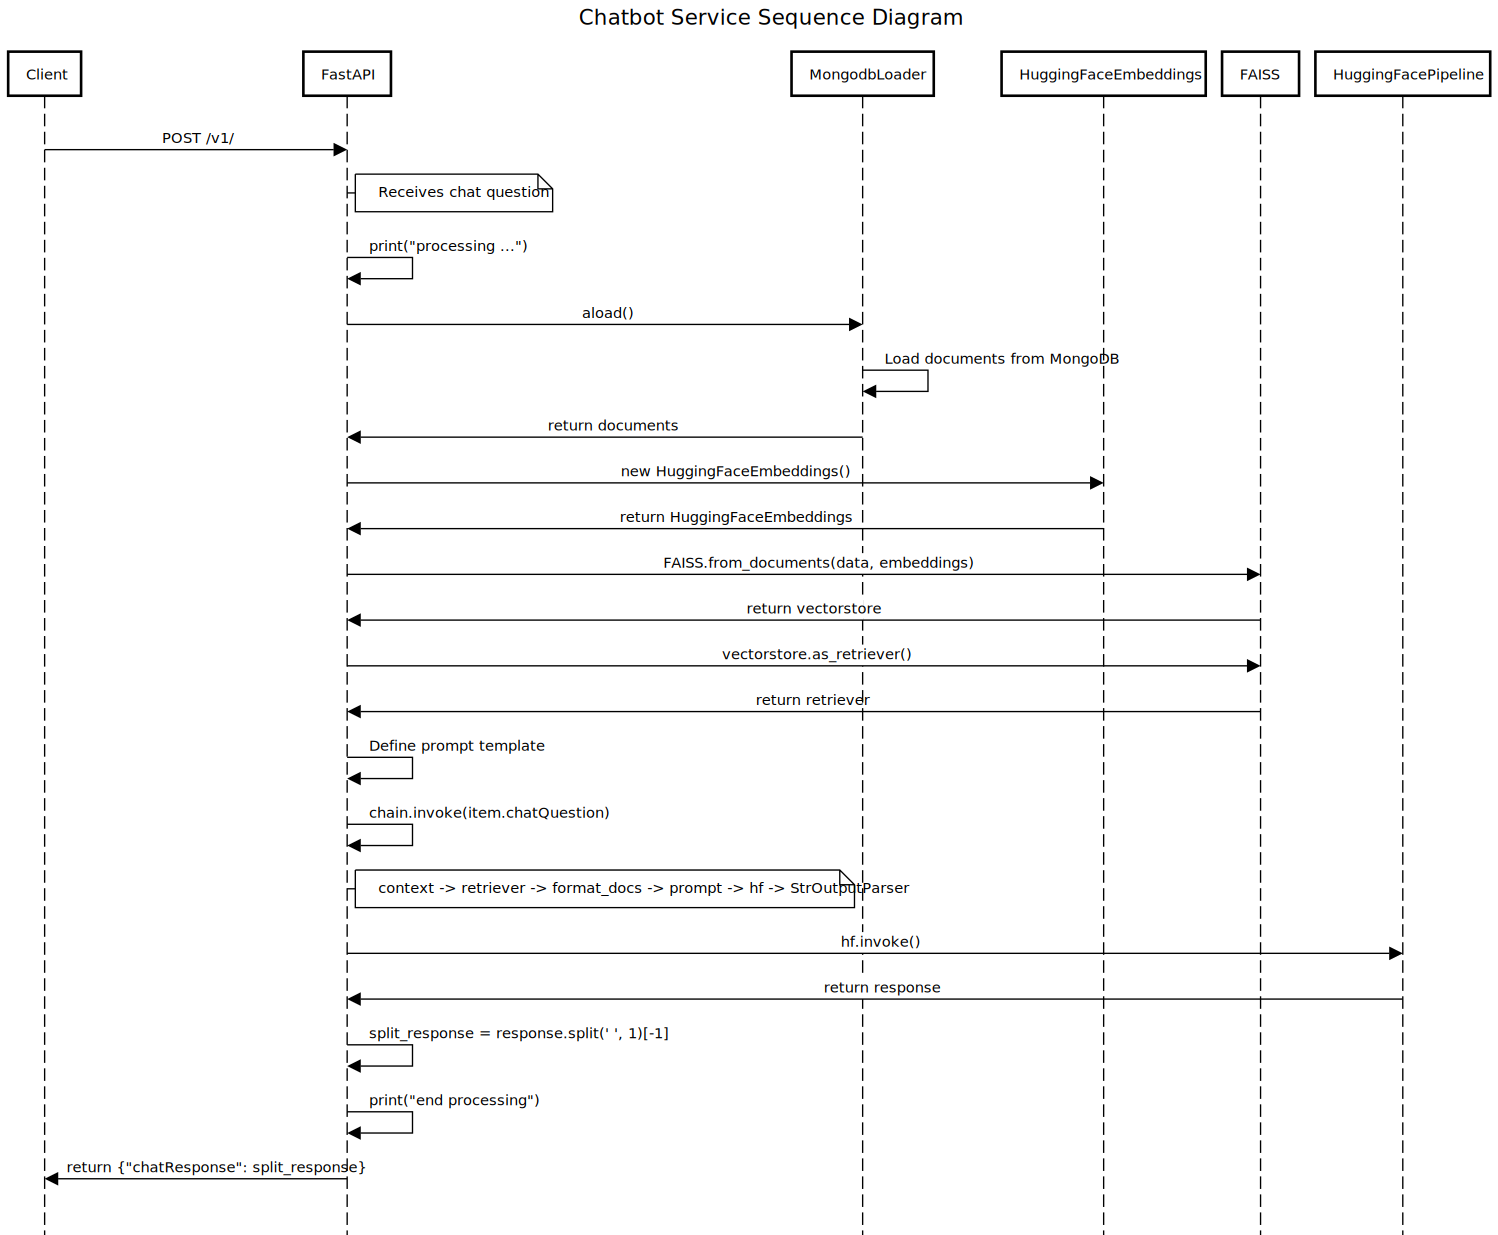
\includegraphics[width=1.2\textwidth]{chatbot-seq.png}
\caption{Diagramme de séquence du sprint 1}
\label{fig:sprint1_seq}
\end{figure}
\FloatBarrier
\section{Réalisation du sprint 1}

% Espace pour inclure des images de chat
\begin{center}
    \includegraphics[width=1\textwidth]{chat1.png}
    \includegraphics[width=1\textwidth]{chat2.png}
\end{center}

L' images ci-dessus montre un exemple de conversation avec le chatbot lors des premiers tests. Ces captures d'écran illustrent la convivialité de l'interface utilisateur et la capacité du chatbot à répondre efficacement aux requêtes des utilisateurs.


Pour le développement du chatbot, le modèle Llama 2 a été utilisé comme base de l'infrastructure de traitement du langage naturel. Llama 2 est un modèle pré-entraîné puissant qui offre des capacités avancées de génération de texte et d'analyse de langage naturel, ce qui en fait un choix idéal pour la création d'un chatbot intelligent et réactif.

Le sprint 1 a posé les bases du développement du chatbot, en mettant en place les fondations nécessaires pour son évolution future. Les retours d'expérience recueillis lors de cette phase ont été précieux pour orienter les prochains travaux et assurer le succès du projet.




\chapter{MISE EN ŒUVRE DU SPRINT 2: Authentification et mise a jour de la base de donnees par l’administrateur}
\section{Introduction}

Dans le cadre du sprint 2, l'équipe s'est concentrée sur authentification et la mise à jour de la base de données par le gestionnaire, conformément à l'User Story 1.3. Cette fonctionnalité permet au gestionnaire d'effectuer des modifications sur les ressources du chatbot via l'application, qui est connectée à MongoDB. Voici les détails de cette étape :

\section{Backlog du Sprint 2}

Le développement de notre application de gestion de chatbot s’est structuré autour d’un backlog produit bien défini, comprenant plusieurs épopées et user stories. Chaque user story a été accompagnée de critères d’acceptation clairs pour garantir la qualité et la conformité aux attentes.

\subsection{Épopée 1 : Authentification et mise à Jour de la Base de Données par l’Administrateur}

\textbf{Authentification se fait par Keycloak}

\textbf{User Story 1.3 : Mise à Jour de la Base de Données par l’Administrateur}
\begin{itemize}
    \item \textbf{En tant que :} administrateur
    \item \textbf{Je veux :} pouvoir mettre à jour la base de données du chatbot à tout moment
    \item \textbf{Afin de :} m’assurer que les informations sont toujours à jour
    \item \textbf{Critères d'acceptation :}
    \begin{itemize}
        \item L’administrateur peut accéder à une interface pour mettre à jour la base de données.
        \item Les modifications sont immédiatement reflétées dans les réponses du chatbot.
    \end{itemize}
\end{itemize}

\subsection{Sprint Plan}
\begin{itemize}
    \item \textbf{Sprint 2 :} Mise à jour de la base de données par l’administrateur (User Story 1.3), Consultation des cours disponibles (User Story 2.1)
\end{itemize}

\section{Analyse et Conception}
\subsection{Description textuel}
\begin{itemize}
    \item **Analyse des Besoins :** L'équipe a étudié les exigences de l'User Story 1.3 pour comprendre les fonctionnalités spécifiques attendues par le gestionnaire. Cela comprenait la capacité de modifier les ressources du chatbot telles que les réponses prédéfinies, les questions fréquemment posées, etc.
    
    \item **Développement de l'Application :** Une application dédiée a été développée, offrant une interface conviviale permettant au gestionnaire d'accéder et de modifier les ressources du chatbot directement via MongoDB. L'application a été conçue pour être sécurisée et intuitive, garantissant une expérience utilisateur optimale.
    
    \item **Intégration avec MongoDB :** L'application a été connectée à MongoDB pour permettre une interaction transparente avec la base de données. Cela a permis au gestionnaire d'accéder aux données du chatbot en temps réel et de les modifier selon ses besoins, sans nécessiter de connaissances techniques avancées.
    
    \item **Tests et Validation :** Une série de tests ont été effectués pour valider la fonctionnalité de mise à jour de la base de données par le gestionnaire. Cela comprenait des tests d'interface utilisateur, des tests de performance et des tests de sécurité pour garantir le bon fonctionnement de l'application dans divers scénarios d'utilisation.
\end{itemize}

\subsection{Diagramme de cas d'utilisation de sprint 2}


\begin{figure}[H]
\centering
\includegraphics[width=\textwidth]{sprint2-usecase.png} 
\caption{Diagramme de cas d'utilisation de sprint 2}
\label{fig:s2_usecase}
\end{figure}

\subsection{Diagramme de classe de sprint 2}
\begin{figure}[H]
\centering
\includegraphics[width=\textwidth]{sprint2-class.png} 
\caption{Diagramme de classe de sprint 2}
\label{fig:s2_class}
\end{figure}

\subsection{Diagramme de séquence de sprint 2}


\begin{figure}[H]
\centering
\includegraphics[width=\textwidth]{keycloak-seq.png} 
\caption{Diagramme de sequence d' authentification par Keycloak}
\label{fig:s2_auth}
\end{figure}


\begin{figure}[H]
\centering
\includegraphics[width=\textwidth]{chat-res-seq.png} 
\caption{Diagramme de s ́equence de sprint 2
}
\label{fig:chatres_seq}
\end{figure}

\section{Realisation}


\begin{figure}[H]
\centering
\includegraphics[width=\textwidth]{admin-doc.png} 
\caption{Capture d'ecrant d'interface qui permet au géstionnaire de modifier la base des resources du chatbot}
\label{fig:screen_chat_res}
\end{figure}

L'image ci-dessus montre un screenshot de l'application développée pour permettre au gestionnaire de modifier les ressources du chatbot via MongoDB. Cette interface conviviale offre une vue claire et intuitive des données, permettant au gestionnaire d'effectuer facilement les modifications nécessaires.

Le sprint 2 a permis de mettre en place une fonctionnalité essentielle pour la gestion et la maintenance du chatbot, en offrant au gestionnaire un moyen simple et efficace de mettre à jour les ressources du chatbot en temps réel.

\newpage


\chapter{MISE EN ŒUVRE DU SPRINT 3: Inscription aux cours, événements et certificats}
\section{Introduction}

Le sprint 3 a été consacré à la mise en œuvre de l'User Story 2.2, qui concerne l'inscription aux cours et événements, ainsi que l'inscription aux examens de certification gratuits. Cette fonctionnalité permet aux utilisateurs de s'inscrire à des cours et événements proposés par le Centre Code 212, ainsi qu'aux examens de certification associés. Voici les détails de cette étape :

\begin{itemize}
    \item \textbf{Analyse des Besoins :} L'équipe a étudié les exigences de l'User Story 2.2 pour comprendre les fonctionnalités spécifiques attendues par les utilisateurs. Cela comprenait la capacité de s'inscrire à des cours, événements et examens de certification directement via la plateforme.
    
    \item \textbf{Développement de l'Application :} Une fonctionnalité dédiée a été développée, offrant une interface conviviale permettant aux utilisateurs de consulter et s'inscrire aux cours, événements et examens de certification. L'application a été conçue pour être sécurisée et intuitive, garantissant une expérience utilisateur optimale.
    
    \item \textbf{Intégration avec le Système de Gestion :} L'application a été connectée au système de gestion pour permettre une interaction transparente avec les données de cours, événements et examens de certification. Cela a permis aux utilisateurs d'accéder aux informations en temps réel et de s'inscrire selon leurs besoins.
    
    \item \textbf{Tests et Validation :} Une série de tests ont été effectués pour valider la fonctionnalité d'inscription aux cours, événements et examens de certification. Cela comprenait des tests d'interface utilisateur, des tests de performance et des tests de sécurité pour garantir le bon fonctionnement de l'application dans divers scénarios d'utilisation.
\end{itemize}

\section{Backlog du Sprint 3}

Le développement de notre application de gestion de chatbot s’est structuré autour d’un backlog produit bien défini, comprenant plusieurs épopées et user stories. Chaque user story a été accompagnée de critères d’acceptation clairs pour garantir la qualité et la conformité aux attentes.

\subsection{Épopée 2 : Inscription aux Cours, Événements et Examens de Certification}

\textbf{User Story 2.2 : Inscription aux Cours et Événements}
\begin{itemize}
    \item \textbf{En tant que :} utilisateur
    \item \textbf{Je veux :} m'inscrire aux cours et événements
    \item \textbf{Afin de :} participer à ceux-ci
    \item \textbf{Critères d'acceptation :}
    \begin{itemize}
        \item Les utilisateurs peuvent s'inscrire à des cours et des événements via la plateforme.
        \item Un système de confirmation d'inscription est en place.
    \end{itemize}
\end{itemize}

\textbf{User Story 2.3 : Inscription aux Examens de Certification Gratuits}
\begin{itemize}
    \item \textbf{En tant que :} utilisateur
    \item \textbf{Je veux :} m'inscrire à des examens de certification gratuits
    \item \textbf{Afin de :} obtenir des certifications
    \item \textbf{Critères d'acceptation :}
    \begin{itemize}
        \item Les utilisateurs peuvent voir les examens de certification disponibles et s'y inscrire gratuitement.
        \item Un système de confirmation d'inscription aux examens est en place.
    \end{itemize}
\end{itemize}


\section{Analyse et Conception}
\subsection{Diagramme de cas d'utilisation de sprint 3}

\begin{figure}[H]
\centering
\includegraphics[width=\textwidth]{sprint3-usecase.png} 
\caption{Diagramme de cas d'utilisation de sprint 3}
\label{fig:s3-use}
\end{figure}

\subsection{Diagramme de classe de sprint 3}

\begin{figure}[H]
\centering
\includegraphics[width=\textwidth]{sprint2-class.png} 
\caption{Diagramme de classe de sprint 3}
\label{fig:s3_class}
\end{figure}

\subsection{Diagramme de Séquence de sprint 3}
\clearpage
\begin{figure}
\centering
\includegraphics[width=\textwidth]{seq-certifs.png} 
\caption{Diagramme de sequence des certificats}
\label{fig:seq_certifs}
\end{figure}

\section{Réalisation}
\begin{figure}
\centering
\includegraphics[width=\textwidth]{admin-add-certif.png} 
\caption{Ajout des certificats par le gestionnaire}
\label{fig:Ajout_des_certificats}
\end{figure}


\begin{figure}
\centering
\includegraphics[width=\textwidth]{certifs-list.png} 
\caption{Liste des certificats disponibles}
\label{fig:certificates}
\end{figure}


\begin{figure}
\centering
\includegraphics[width=\textwidth]{calendar.png} 
\caption{Le calendrier de l'étudiant avec les événements auxquels il est inscrit}
\label{fig:calender}
\end{figure}



\clearpage

\chapter{MISE EN ŒUVRE DU SPRINT 4: Amélioration de l’Interface Utilisateur et  d ́eploiment et creation des contenaires}


\section{Introduction}
Le sprint 3 a été consacré à l'amélioration de l'interface utilisateur (UI) et à l'optimisation des performances du chatbot, conformément aux User Stories 3.1 et 3.2. Cette phase a visé à améliorer l'expérience globale des utilisateurs et à garantir des performances optimales du chatbot. De plus, dans ce sprint, des conteneurs Docker ont été créés pour chaque service, facilitant ainsi le déploiement et la gestion de l'ensemble du système. Voici les détails de cette étape :


\section{Backlog du Sprint 4}

Le développement de notre application de gestion de chatbot s’est structuré autour d’un backlog produit bien défini, comprenant plusieurs épopées et user stories. Chaque user story a été accompagnée de critères d’acceptation clairs pour garantir la qualité et la conformité aux attentes.

\subsection{Épopée 2 : Développement des Fonctionnalités de la Plateforme}

\textbf{User Story 2.2 : Inscription aux Cours et Événements}
\begin{itemize}
    \item \textbf{En tant que :} utilisateur
    \item \textbf{Je veux :} m'inscrire aux cours et événements
    \item \textbf{Afin de :} participer à ceux-ci
    \item \textbf{Critères d'acceptation :}
    \begin{itemize}
        \item Les utilisateurs peuvent s'inscrire à des cours et des événements via la plateforme.
        \item Un système de confirmation d'inscription est en place.
    \end{itemize}
\end{itemize}

\textbf{User Story 2.3 : Inscription aux Examens de Certification Gratuits}
\begin{itemize}
    \item \textbf{En tant que :} utilisateur
    \item \textbf{Je veux :} m'inscrire à des examens de certification gratuits
    \item \textbf{Afin de :} obtenir des certifications
    \item \textbf{Critères d'acceptation :}
    \begin{itemize}
        \item Les utilisateurs peuvent voir les examens de certification disponibles et s'y inscrire gratuitement.
        \item Un système de confirmation d'inscription aux examens est en place.
    \end{itemize}
\end{itemize}


\section{Analyse et Conception}
\subsection{Description textuel}
\begin{itemize}
    \item **Optimisation des Performances du Chatbot :** L'équipe a effectué une série d'optimisations pour améliorer le temps de réponse du chatbot. Cela comprenait des ajustements dans l'architecture du modèle, l'optimisation des requêtes et l'amélioration globale de l'efficacité des processus de traitement du langage naturel.
    
    \item **Amélioration de l'Interface Utilisateur :** L'interface utilisateur du chatbot a été revue et améliorée pour offrir une expérience plus conviviale et esthétique. Des fonctionnalités telles que le mode sombre et le mode clair ont été ajoutées pour permettre aux utilisateurs de choisir leur préférence visuelle. De plus, des animations ont été intégrées pour rendre l'interface plus dynamique et engageante.
    
    \item **Création des Conteneurs Docker :** Dans le cadre de la préparation au déploiement, des conteneurs Docker ont été créés pour chaque service du système. Cela inclut le chatbot, le service web, la base de données et tout autre composant nécessaire. Les conteneurs Docker offrent une méthode standardisée et portable pour empaqueter, distribuer et exécuter des applications, simplifiant ainsi le processus de déploiement et de gestion.
    
    \item **Tests de Performance et de Convivialité :** Des tests approfondis ont été effectués pour évaluer l'impact des améliorations apportées à l'interface utilisateur et aux performances du chatbot. Cela comprenait des tests de charge pour évaluer la stabilité du système sous charge maximale, ainsi que des tests d'utilisabilité pour évaluer la facilité d'utilisation de l'interface par les utilisateurs finaux.
\end{itemize}

Le sprint 4 a permis d'apporter des améliorations significatives à l'expérience utilisateur et aux performances du chatbot, tout en préparant le système à un déploiement efficace à l'aide de conteneurs Docker.

\subsection{Screenshots}

\begin{figure}
\centering
\includegraphics[width=\textwidth]{light-chat.png} 
\caption{Chat bot en light mode}
\label{fig:lightchat}
\end{figure}


\begin{figure}
\centering
\includegraphics[width=\textwidth]{light-profile.png} 
\caption{Le profile d'utilisateur en light mode}
\label{fig:profile}
\end{figure}

\clearpage


\section{Déploiement et Infrastructure}
Le déploiement des microservices a été réalisé à l'aide de conteneurs Docker, assurant une portabilité et une isolation des services. Docker a été choisi en raison de sa capacité à empaqueter les applications et leurs dépendances de manière cohérente, garantissant que les services fonctionnent de manière identique sur n'importe quel environnement. 

Un Docker Compose a été créé pour orchestrer les différents services et simplifier le déploiement de l'ensemble de l'application. Cette approche permet de définir et de gérer les services, les réseaux et les volumes dans un fichier YAML unique, facilitant ainsi le déploiement et la mise à l'échelle des microservices.

Kubernetes a été utilisé pour l'orchestration des conteneurs, permettant une gestion automatisée du déploiement, de la mise à l'échelle et de la maintenance des applications conteneurisées. Kubernetes a été choisi pour sa robustesse, sa capacité à gérer des déploiements complexes et son large écosystème de support. Il permet également de s'assurer que les applications sont hautement disponibles et peuvent se redimensionner en fonction des besoins.

\subsection{Environnement de Production}
L'environnement de production a été configuré pour garantir une haute disponibilité et une résilience face aux pannes. Des pratiques de surveillance et de logging ont été mises en place pour assurer une surveillance proactive et une résolution rapide des incidents. Kubernetes facilite également la mise en place d'un environnement de production résilient grâce à ses capacités de gestion des défaillances et de répartition de charge.

\subsection{Sécurité}
Des mesures de sécurité ont été intégrées dès le début du développement, incluant l'utilisation de Keycloak pour la gestion des accès, la mise en place de pare-feu, et l'utilisation de certificats SSL pour les communications sécurisées. L'utilisation de Kubernetes ajoute une couche supplémentaire de sécurité grâce à ses fonctionnalités natives, telles que la gestion des secrets et la définition de politiques de sécurité au niveau du cluster.



\section{Conclusion}
La réalisation et la mise en œuvre de l'application ont suivi une approche structurée et méthodique, garantissant le respect des délais et des exigences de qualité. L'utilisation de la méthodologie agile, combinée à des technologies modernes et des pratiques de déploiement robustes, a permis de développer une application modulaire, scalable et sécurisée, répondant aux besoins des utilisateurs finaux.


\chapter{Conclusion Générale}

Ce rapport résume notre travail durant notre stage de fin d’année au sein du centre Code212. Nous avons commencé par introduire le contexte général du projet et les différents besoins et exigences, puis nous avons préparé un planning de travail en respectant les priorités des besoins. Nous avons consacré la partie suivante à l’étude technique et aux choix des outils et technologies. Ensuite, nous avons entamé la réalisation de chaque sprint.
\newline
Ce projet a eu pour objectif principal de développer et implémenter un chatbot doté d'intelligence artificielle au sein de la plateforme e-learning de Code212. Cette initiative s'inscrit dans le contexte d'une digitalisation croissante de l'éducation, nécessitant des outils innovants et réactifs pour répondre efficacement aux besoins des étudiants. Code212, en tant qu'acteur clé dans la formation numérique au Maroc, vise par cette démarche à améliorer l'interaction et l'assistance offertes à ses apprenants, tout en optimisant ses ressources pédagogiques.
\newline

L'introduction du chatbot IA apporte des bénéfices multiples. Les étudiants bénéficient d'une assistance instantanée pour leurs questions fréquentes, ce qui facilite un apprentissage autonome et renforce le processus éducatif. En fournissant des outils pratiques et interactifs pour la formation, Code212 prépare mieux ses étudiants à intégrer le marché du travail numérique. De plus, le chatbot aide à une utilisation plus efficace des ressources pédagogiques disponibles, maximisant ainsi l'efficacité des études des apprenants. En offrant un soutien empathique et motivant, le chatbot contribue à maintenir la persévérance et l'engagement des étudiants.

Cependant, le projet n'a pas été exempt de défis. La conception d'un système AI convivial a été surmontée par une compréhension précise des besoins des utilisateurs et par des itérations continues basées sur les feedbacks. L'intégration des technologies de pointe a été gérée efficacement grâce à une planification rigoureuse et à l'adoption de méthodologies Agiles.
\newline

Le succès initial du chatbot IA ouvre de nouvelles perspectives pour Code212. Parmi les pistes de développement futur, on envisage l'élargissement des fonctionnalités en ajoutant des capacités plus avancées comme l'analyse prédictive pour anticiper les besoins des étudiants et offrir des suggestions proactives. Il est aussi envisagé d'intégrer le chatbot à d'autres systèmes éducatifs, connectant ainsi des plateformes d'apprentissage en ligne et des outils de gestion académiques pour une expérience d'apprentissage encore plus fluide. L'amélioration continue basée sur les retours des utilisateurs et les développements technologiques sera essentielle pour rester à la pointe de l'innovation éducative. L'optimisation du chatbot, en recherchant des méthodes pour améliorer les performances, y compris l'optimisation des algorithmes et l'utilisation de technologies de pointe pour réduire les temps de réponse, est également cruciale. Enfin, la mise en œuvre de techniques d'équilibrage de charge pour assurer une répartition efficace des demandes sur les serveurs garantira la disponibilité et la réactivité du chatbot même en période de forte affluence.
\newline

En conclusion, l'intégration d'un chatbot IA au sein de Code212 représente une avancée significative dans l'effort continu de modernisation et d'optimisation de l'éducation numérique au Maroc. Cette initiative répond non seulement aux besoins immédiats des étudiants mais pose également les jalons pour un avenir où l'apprentissage est résolument aligné avec les opportunités et défis du monde numérique. Ainsi, Code212 confirme sa mission de former des professionnels qualifiés et prêts à relever les défis de l'économie numérique, tout en renforçant son rôle de leader dans la transformation digitale de l'enseignement au Maroc.



\chapter*{Bibliographies et Webographie}

\begin{itemize}
    \item[1.] Jeff Sutherland and Ken Schwaber, "Scrum: A Comprehensive Guide to Agile Project Management", 3rd Edition, 2022.
    \item[2.] Guide de démarrage Scrum | L'Agiliste.
    \item[3.] \url{https://www.redhat.com/en/topics/integration/whats-the-difference-between-soaprest}
    \item[4.] \url{https://www.researchgate.net/figure/Client-server-architecture-and-technologies_fig1_353325675}
    \item[5.] \url{https://medium.com/@mindfiresolutions.usa/advantages-and-disadvantages-of-php-frameworks-c046d50754e5}
    \item[6.] \url{https://www.javatpoint.com/advantages-and-disadvantages-of-java}
    \item[7.] \url{https://en.wikipedia.org/wiki/Python_(programming_language)}
    \item[8.] \url{https://www.agilites.com/pros-and-cons-of-using-c-as-your-backend-programming-language.html}
    \item[9.] \url{https://medium.com/@mindfiresolutions.usa/advantages-and-disadvantages-of-php-frameworks-c046d50754e5}
    \item[10.] \url{https://www.javatpoint.com/advantages-and-disadvantages-of-java}
    \item[11.] \url{https://python.plainenglish.io/the-pros-and-cons-of-using-python-for-web-development-9134f2c4f16f}
    \item[12.] \url{https://en.wikipedia.org/wiki/Apache_Maven}
    \item[13.] \url{https://en.wikipedia.org/wiki/Apache_Ant}
    \item[14.] \url{https://en.wikipedia.org/wiki/Gradle}
    \item[15.] Laurentiu Spilca, "Spring Security in Action".
    \item[16.] Kim Hamilton and Russ Miles, "Learning UML 2.0".
    \item[17.] \url{https://www.amigoscode.com/p/spring-boot-security}
    \item[18.] \url{https://en.wikipedia.org/wiki/Spring_Framework}
    \item[19.] \url{https://en.wikipedia.org/wiki/Spring_Framework#Spring_Boot}
    \item[20.] \url{https://en.wikipedia.org/wiki/Spring_Security}
    \item[21.] \url{https://www.infoq.com/articles/spring-data-intro/}
    \item[22.] \url{https://en.wikibooks.org/wiki/Java_Persistence/What_is_JPA%3F}
    \item[23.] \url{https://www.javatpoint.com/hibernate-tutorial}
    \item[24.] \url{https://fr.wikipedia.org/wiki/IntelliJ_IDEA}
    \item[25.] \url{https://www.blazemeter.com/blog/how-use-postman-manage-and-execute-your-apis}
    \item[26.] \url{https://en.wikipedia.org/wiki/Swagger_(software)}
    \item[27.] Craig Walls, "Spring in Action, Fifth Edition".
    \item[28.] \url{https://blog.logrocket.com/tailwind-css-is-it-tomorrows-bootstrap-ebe560f9d00b/}
    \item[29.] \url{https://fr.wikipedia.org/wiki/Bootstrap_(framework)}
    \item[30.] \url{https://en.wikipedia.org/wiki/HTML}
    \item[31.] \url{https://en.wikipedia.org/wiki/CSS}
    \item[32.] \url{https://en.wikipedia.org/wiki/JavaScript}
    \item[33.] \url{https://dev.to/cesareferrari/working-with-axios-in-react-540c}
    \item[34.] \url{https://en.wikipedia.org/wiki/JSON}
    \item[35.] \url{https://www.journaldev.com/10660/json-server}
    \item[36.] \url{https://en.wikipedia.org/wiki/Git}
    \item[37.] \url{https://en.wikipedia.org/wiki/GitHub}
    \item[38.] \url{https://en.wikipedia.org/wiki/GanttProject}
    \item[39.] \url{https://en.wikipedia.org/wiki/MySQL}
    \item[40.] \url{https://en.wikipedia.org/wiki/PostgreSQL}
    \item[41.] \url{https://huggingface.co/} - Hugging Face, plateforme pour les modèles de langage et les outils NLP.
    \item[42.] \url{https://langchain.com/} - LangChain, une bibliothèque pour la création d'applications alimentées par des modèles de langage.
    \item[43.] \url{https://github.com/facebookresearch/llama} - LLaMA 2, un modèle de langage de Facebook AI Research.
    \item[44.] \url{https://fastapi.tiangolo.com/} - FastAPI, un framework web pour Python pour la construction d'API rapides et performantes.
\end{itemize}


\end{document}




